\documentclass[a4paper,final,12pt]{report}
\newcommand\tab[1][13mm]{\hspace*{#1}}
\usepackage[english]{babel}
\usepackage{times}
\usepackage[left=4cm,right=4cm]{geometry}
\usepackage{geometry} % Deve esserci!
\usepackage{graphicx} % permette di inserire immagini
\usepackage[table,xcdraw]{xcolor}
\usepackage{longtable}
\usepackage{amsmath, amssymb, cite}
\usepackage{booktabs}
\usepackage{listings}
\usepackage{algorithm}
\usepackage{algorithmic}
\usepackage{url}
\usepackage{caption}
\setcounter{tocdepth}{4}


% Comandi per impaginare secondo le regole Unibo, da mettere dopo gli usepackage
\renewcommand{\baselinestretch}{1.25}
\newlength{\alphabet}
\settowidth{\alphabet}{\normalfont abcdefghijklmnopqrstuvwxyz}
\newgeometry{textwidth=2.5\alphabet,lines=35}

\begin{document}
\newenvironment{dedication}
{\clearpage           % we want a new page
  \pagenumbering{gobble}
  \thispagestyle{empty}% no header and footer
  \vspace*{\stretch{1}}% some space at the top 
  \itshape             % the text is in italics
  \raggedleft          % flush to the right margin
}
{\par % end the paragraph
  \vspace{\stretch{3}} % space at bottom is three times that at the top
  \clearpage           % finish off the page
  \pagenumbering{arabic}
}

% Frontespizio
\newgeometry{hmarginratio=1:1}
\begin{titlepage}
  \begin{center}
  %{{\Large{\textsc{Alma Mater Studiorum - Università di
  %Bologna}}}}\\
    \begin{figure}[hbtp]
    \centering
    \includegraphics[scale=1]{img/logo.png}
    \end{figure}

  \vspace{5mm}
  {\small Dipartimento di Informatica - Scienza e Ingegneria \\
  Corso di Laurea Magistrale in Ingegneria e Scienze Informatiche}
  \end{center}
  
\vspace{12mm}
\begin{center}
{\Large\textsc{\raggedright{Predictive Modeling of Tire Grip During Cornering in High-Speed Racing}}}\
\end{center}
\vspace{20mm}
\par
\noindent
  
  \begin{center}
    \large{Elaborato in \\
    Smart Vehicular Systems}
  \end{center}
  \vspace{15mm}
  \par
  \noindent
  
  \begin{minipage}[t]{0.47\textwidth}
  {\large{\bf Relatrice:\\
  Silvia Mirri
  \\}}
  {\large{\bf Correlatori:\\
  Roberto Girau\\
  Giovanni Pau
  }}
  \end{minipage}
  \hfill
  \begin{minipage}[t]{0.47\textwidth}\raggedleft
  {\large{\bf Presentata da:\\
  Andrea Bedei}}
  \end{minipage}
  \vspace{7mm}
  \begin{center}
  {\large{\bf Sessione Luglio 2025\\ Anno Accademico 2024/2025}}
  \end{center}
\end{titlepage}

\restoregeometry
\clearpage\null\thispagestyle{empty}\newpage

\cleardoublepage

% Inserisci frase e ringraziamenti
    \begin{flushright}
    \thispagestyle{empty}
    \null\vspace{\stretch {1}}
    \emph{I have a dream.\break --- Martin Luther King Jr.}
    \vspace{\stretch{2}}\null
    \end{flushright}
    \cleardoublepage
    
    \clearpage\null\thispagestyle{empty}\newpage
    
    \begin{abstract}
    Abstract
    \end{abstract}
    
    
    \setlength{\parindent}{0pt}
    \begin{LARGE}
    \textbf{Thanksgiving\\\\}
    \end{LARGE}
    \tab[10pt] I am proud to dedicate this space of my paper to the people who supported me in the writing of my thesis and throughout my entire degree. I am convinced that, without them, I would not have made it this far.\\
    \tab[10pt] First and foremost, I thank my thesis advisor, who throughout my academic journey has always helped me with great professionalism and extreme helpfulness.\\
    \tab[10pt] I thank my parents, who have supported me throughout my academic journey, because without them I would not have made it. \\
    \tab[10pt] In particular, I thank my sister, who has always been there in times of need.\\
    \tab[10pt] Special thanks go to my grandmother, who has always believed in me and supported me at every moment of my academic journey and life.\\
    \tab[10pt] I thank all my friends, who have been there for me, supported me and put up with me at every stage of our lives. Special thanks go to Fabio, without whom I probably would not have enrolled in college. I also thank Lorenzo and Giulia, who have always been by my side. Special thanks also go to Matteo, who has always supported me at times when I really needed it. Finally, I thank Giuseppe, Mattia, Nicholas and Sara, whose advice made my life easier. 

\tableofcontents
\listoffigures
\listoftables
%\lstlistoflistings
\setlength{\parindent}{0pt}

\chapter{Introduction}
\section{The Environment}
This dissertation has been developed in collaboration with the Technology Innovation Institute (TII), which is a leading research institution based in Abu Dhabi, United Arab Emirates \cite{TII}. The TII focuses on the advancement of innovative technologies in various fields, including artificial intelligence, robotics, and autonomous systems. Among its most recognized initiatives is the design and development of fully autonomous Formula 1 (F1) racing cars. \cite{AutonomousRacing}.

The TII project is about creating intelligent systems that can compete with human drivers in high-speed motorsport environments independently. This entails putting professional drivers' abilities and decision-making powers into the form of a computer program that can process huge amounts of information in real time, adapt circuit by circuit, and make optimisation choices for itself \cite{AI_F1}. Its purpose is to push AI-enhanced motorsport and bring the envelope nearer to mass-deployed autonomous vehicles.

Autonomous racing involves numerous challenges, such as high speed decision making, real time sensor fusion, and dynamic adaptation to the environment's conditions. The AI models trained for this must process a real time stream of data, such as:
\begin{itemize}
    \item Forces on the car and the driver
    \item Tire temperature and pressure,
    \item Speed and acceleration,
    \item Grip levels on various track surface.
\end{itemize}
Using reinforcement and machine learning algorithms, the system learns to drive the track optimally, balancing acceleration, braking, and steering in the way a human driver would, by simulating the decision making process of the latter. The ultimate hope is to create AI models that can compete at world level and outscore human drivers in terms of efficiency and accuracy \cite{SelfDriving}.

The significance of the study is not only in racing, as it develops autonomous driving technology that can be transferred to real world transportation systems. The insights gained from autonomous F1 racing are applied to enhance algorithms for autonomous vehicles, which become safer, more responsive, and more adaptive to difficult driving conditions \cite{SelfDriving}.

\section{The Issue}
The main aim of this research is to create a system that uses sensors embedded in a fully autonomous Formula 1 vehicle to enable the creation of an artificial intelligence model that can determine the possibility of achieving optimal vehicle performance in cornering \cite{AI_F1}. Specifically, in the cornering stage, the system must calculate the different forces acting on the vehicle and analyze the surroundings to decide whether to accelerate or use the brakes, thus seeking to reduce cornering time while staying within the vehicle's operating parameters.

This means that the autonomous racing agent incorporates an additional decision making factor, allowing it to evaluate the need for greater acceleration or braking in cornering maneuvers, based on all available sensor information \cite{AutonomousRacing}. These decisions have to be implemented by an artificial intelligence model in real time, thus ensuring that the car remains stable and does not exceed its traction limits.

This problem is generally referred to as the \textbf{Grip Problem}, since the decision process is focused on maintaining vehicular control. The vehicle needs to have sufficient grip to stay in contact with the road while optimizing its speed in the turn. Thus, the artificial intelligence needs to determine on its own whether to slow down or speed up, depending on the current status of the vehicle \cite{SelfDriving}.

\section{Understanding Grip in Cornering Dynamics}
Grip, or \textit{tire road friction}, is the fundamental force that allows a vehicle to maintain control while navigating a turn.  It is mainly described by the \textbf{friction coefficient ($\mu$)} between the tires and the road surface, which in turn depends on factors such as tire composition, temperature, vertical load ($F_z$), roadway surface conditions. \cite{Pacejka2012}.

\subsection{Grip is a temporal phenomenon}
Grip depends on the evolution of conditions over time, such as:
\begin{itemize}
    \item \textbf{Forces acting on the car (G force):} influence the stability and behavior of the car.
    \item \textbf{Tyre pressure and temperature:} change over the seconds and influence grip.
    \item \textbf{Speed and steering angle:} grip changes with the driver's input and track conditions.
\end{itemize}


\subsection{Physical and Mathematical Definition of Grip}
Grip is described by the equation:
\begin{equation}
    F_y = \mu F_z
\end{equation}
where:
\begin{itemize}
    \item $F_y$ is the lateral force resisting centrifugal forces when turning,
    \item $\mu$ is the tire road friction coefficient. It depends on road texture and rubber properties,
    \item $F_z$ is the vertical load on the tire, which is influenced by vehicle weight and aerodynamics.
\end{itemize}
The lateral grip is what makes a car move in a curved trajectory without flipping over. If $F_y$ exceeds the available grip force, the car will \textbf{understeer} (front wheels lose grip) or \textbf{oversteer} (rear wheels lose grip), leading to a loss of control \cite{Milliken1995}.

\subsection{Grip Evolution in a Time Series Framework}
Grip is a dynamic property, not a fixed one; it changes dynamically as the vehicle progresses through a turn. This change can be modeled with a \textbf{time series model}, where:
\begin{itemize}
    \item \textbf{Grip buildup phase:} when the vehicle is entering the corner, the lateral force ($F_y$) increases with slip angle ($\alpha$), following a \textbf{near linear} relationship.
    \item \textbf{Grip saturation phase:} when $F_y$ approaches the peak force ($F_{y,max}$), the tire enters a \textbf{nonlinear} regime where additional slip results in diminishing grip gains.
    \item \textbf{Grip loss phase:} under the application of high lateral force, $F_y$ starts to decrease due to rubber hysteresis and road tire separation, leading to full tire saturation.
\end{itemize}
Mathematically, this is described using Pacejka's Magic Formula.

\chapter{State of the Art}

\section{The Autonomous Racing Car \cite{motor1}}
In autonomous motor racing, the cars used are built on the Dallara Super Formula chassis, which is a high performance open wheel vehicle originally designed for the Japanese Super Formula championship. Unlike their manually driven versions, the cars used in this scenario are equipped with a full autonomous driving system. The drivetrain is a 2.0 liter turbocharged four cylinder Honda engine, rated at around 550 horsepower.

\subsection{Sensor Suite and Data Processing}

Instead of the human operating abilities of the vehicle, the autonomous racing cars use the unique infrastructure called the \textbf{Skid} that supports the suite of sensors making autonomous travel possible. The core sensing elements include:
\newpage
\begin{itemize}
    \item \textbf{Four radar sensors}: are used to measure distances to nearby objects and to detect moving objects.
    \begin{figure}[hbtp]
    \centering
    \includegraphics[scale=0.3]{img/radarUnit.png}
    \caption{Radars are used to measure distances to the nearby objects. \cite{AbuDhabiRacing2024}}
    \label{figura:radarUnit}
    \end{figure}
    
    \item \textbf{Three LiDAR (Light Detection and Ranging) units}: provide a high resolution 3D map of the surroundings, aiding in obstacle detection and environmental mapping.
    \begin{figure}[hbtp]
    \centering
    \includegraphics[scale=0.215]{img/lidarSensor.png}
    \includegraphics[scale=0.195]{img/lidar2.png}
    \caption{The systems provide a 3D map of the surroundings. \cite{AbuDhabiRacing2024}}
    \label{figura:lidarSensor}
    \end{figure}

    \newpage
    \item \textbf{Seven high resolution cameras}: Capture visual data, used for image recognition, object classification, and lane detection.
    \begin{figure}[hbtp]
    \centering
    \includegraphics[scale=0.3]{img/cameras.png}
    \caption{Cameras are used for image recognition, object classification, and lane detection. \cite{AbuDhabiRacing2024}}
    \label{figura:cameras}
    \end{figure}

    \item \textbf{Two GPS sensors}: To track the car in all the circuit. 
    \begin{figure}[hbtp]
    \centering
    \includegraphics[scale=0.218]{img/frontgps.png}
    \includegraphics[scale=0.20]{img/centergps.png}
    \caption{Placement of the front and center GPS sensors used for real time positioning and trajectory optimization \cite{AbuDhabiRacing2024}.}
    \label{figura:gps}
    \end{figure}
\end{itemize}

The detailed information gathered from the sensors is relayed to an advanced onboard computer that interprets the data in real time to determine the most appropriate maneuvers to drive. The central processor serves as the vehicle's \textit{brain}, running advanced artificial intelligence algorithms that analyze sensor information and make decisions on control.
\begin{figure}[hbtp]
\centering
\includegraphics[scale=0.35]{img/computer2.png}
\includegraphics[scale=0.36]{img/Computer.png}
\caption{The Car Computer \cite{AbuDhabiRacing2024}.}
\label{figura:computer}
\end{figure}

\subsection{Telemetry and Sensor Challenges}
There exist additional categories of sensors. Specifically, these other sensors are designed to measure various parameters, including engine revolutions per minute (RPM), brake temperature, tire pressure, aerodynamic loads, and numerous other performance metrics. In modern autonomous racing, telemetry plays an even more critical role, providing real time feedback to AI models responsible for decision making on the track.

A major challenge faced by telemetry systems is the extreme operating environments to which they are exposed. The racing environment exposes the sensors to extreme temperature variations, high level vibrations, and mechanical shocks that are capable of either altering the accuracy and lifetime of the sensors. Moreover, the high levels of data generated from various sensors require effective processing and communication that do not introduce latency in order to support real time decision making.

\subsubsection{Reliability and Sensors Degradation}
The reliability of sensors in high stakes racing environments is crucial for the accurate gathering of information. The major challenges that affect the effectiveness of sensors include:
\begin{itemize}
    \item \textbf{Thermal Stress: }the temperature differences encountered within a racing car can reach astonishing levels, with brake discs reaching temperatures over 1000 degrees Celsius, engine components operating under severe thermal stress, and rapid cooling being assisted by airflow. Such thermal fluctuations cause expansion and contraction of materials, thereby exerting stress on sensor devices. Prolonged exposure to these adverse conditions results in sensor drift, defined as a time dependent loss of measurement accuracy 
    \cite{thermal_sensors}.
    \item \textbf{Vibrational Impact: }Race cars are subjected to continuous vibrations from the engine, aerodynamics, and the quality of the track surface. High frequency vibrations can cause mechanical fatigue in sensor components, leading to gradual degradation in performance or outright failure. To mitigate these effects, sensors must be mounted using vibration dampening materials and be built with significant mechanical robustness \cite{vibration_sensors}.
    \item \textbf{Material Degradation and Environmental Exposure: }apart from exposure to heat and vibration, sensors are exposed to many contaminants like dust, oil, moisture, and debris from the race environment. Such pollutants can lead to corrosion, electrical shorts, or interfere with the accuracy of sensor measurements. To increase the life of sensors, protective coatings, sealed housings, and high tech composite materials are often used \cite{sensor_protection}.
\end{itemize}

\subsubsection{Managing the Volume of Telemetry Data}
A modern autonomous racing car is equipped with dozens of sensors, each generating large amounts of data per second. This scenario poses significant challenges in the areas of data collection, processing, and transmission. The main considerations involved include: 
\begin{itemize}
    \item \textbf{Real Time Data Processing: }telemetry data has to be processed in real time in order to enable timely feedback for artificial intelligence powered control systems. This requires the availability of high speed onboard computing units with parallel processing capabilities, often using FPGA (Field Programmable Gate Arrays) or GPUs to handle the high computational requirements \cite{real_time_processing}.
    \item \textbf{Data Transmission Bottlenecks: }optimization of the transmission process of large telemetry datasets is necessary to reduce latency problems. Typically used wireless communication protocols are ultra wideband (UWB) telemetry and high speed optical fiber links. Because of limitations related to bandwidth, it is important to use advanced data compression techniques and to prioritize essential data streams \cite{data_transmission}.
    \item \textbf{Data Storage and Long Term Analysis: }in order to enable post race analysis, it is important that high resolution telemetry data is stored in an optimal fashion. Distributed storage systems with cloud based analytical platforms are usually used to handle the large datasets generated over many races. Advanced artificial intelligence techniques like predictive analytics and anomaly detection are used to obtain useful insights from this data \cite{data_storage}.
\end{itemize}

\subsection{Decision Making and Vehicle Control}
The commands generated by the unified artificial intelligence are sent to the \textbf{Behavioral Supervisory Unit (BSU)} that acts as the sub control mechanism responsible for carrying out the needed driving actions. The BSU will interact with the vehicle’s:
\begin{itemize}
    \item \textbf{Steering actuators}: control the direction of the front wheels according to decisions of artificial intelligence.
    \item \textbf{Braking system}: Engages or releases the brakes to control speed and manage deceleration in corners.
    \item \textbf{Throttle actuators}: Modulate acceleration based on real time conditions and grip levels.
\end{itemize}

\subsection{Autonomous Driving Levels}
The Society of Automotive Engineers (SAE) classifies driving automation into six levels, from Level 0 to Level 5.
\begin{itemize}
    \item \textbf{Level 0}: no automation exists; the responsibility of performing every function rests on the human driver.
    \item \textbf{Level 1}: driver support; the vehicle is able to support either steering or accelerating/deceleration but not at the same time.
    \item \textbf{Level 2}: partial automation; the vehicle can control both steering and acceleration/braking, but a human driver must remain engaged.
    \item \textbf{Level 3}: this level refers to conditional automation, where the car can handle all driving tasks under specific conditions; however, it requires human input when requested by the system.
    \item \textbf{Level 4}: widespread automation; the car can operate independently in designated environments, without the need for human intervention.
    \item \textbf{Level 5}: Full automation; the car can drive itself under all environmental conditions without any human intervention.
\end{itemize}

The autonomous cars used in autonomous racing fall under the category of \textbf{Level 4} autonomous vehicles. This is because of their capacity to move on their own on a pre determined racetrack independently of human intervention. However, unlike Level 5 systems, the cars are limited to controlled situations and rely on preprogrammed paths.

\subsection{Deterministic vs Non Deterministic Decision Making}
An essential distinction in the management structure of these vehicles is the nature of decision making at multiple levels of computation:
\begin{itemize}
    \item The \textbf{high level AI system} operates in a \textbf{non deterministic} manner. This means that its decision making is not fixed; instead, it develops according to changing circumstances. The AI continually refines its control methods through the use of reinforcement learning and data driven algorithms.
    \item The \textbf{BSU (Behavioral Supervisory Unit)} is \textbf{deterministic} in its approach. It uses preprogrammed responses to manage inputs and uphold safety constraints to ensure consistent behavior and immediate responses to failures in the system or unexpected events.
\end{itemize}

The deployment of deterministic and non deterministic processing allows the self racing car to realize an optimum balance between adaptability and safety to guarantee superior performance in conjunction with strong control.

\section{AI Agents in Decision Making for Autonomous F1 Cars}
AI agents in autonomous racing cars function as intelligent systems. The systems utilize sensors, cameras, and computational programs to interpret the environment, make decisions, and interact with the racetrack conditions dynamically \cite{allaboutai}.

\begin{figure}[hbtp]
\centering
\includegraphics[scale=0.3]{img/AiAgents.png}
\caption{The systems utilize sensors, cameras, and computational programs to interpret the environment, make decisions, and interact. \cite{allaboutai}}
\label{figura:AIAgent}
\end{figure}

In a MAS, many artificial intelligence agents are assigned specific tasks, such as steering, braking, grip estimation and traction control. This cooperative work ensures proper monitoring and responsibleness in complicated racing situations.

The structured decision making process in an autonomous F1 car involves multiple layers of data collection and analysis. MAS distributes workloads across agents, enhancing system efficiency.

\subsection{Grip Estimation Agent}
The grip estimation agent continuously monitors the tire surface interactions using sensor fusion techniques, including:
\begin{itemize}
    \item Tire pressure and temperature measuring sensors
    \item Accelerometers and gyroscopes
    \item Assessment of road conditions using combined cameras.
\end{itemize}
The sensors together measure the coefficient of friction, which allows the artificial intelligence system to adapt its acceleration and braking strategies \cite{toyota_research}.

\subsection{Traction Control Agent}
The traction control system prevents excessive wheel slip by dynamically apportioning power to the wheels through regulation.
\begin{itemize}
    \item Torque vectoring algorithms for real time applications.
    \item Differential braking strategies
    \item The application of reinforcement learning to improve power utilization in curves 
\end{itemize}

\subsection{High Frequency Sensor and Data Management}
A significant challenge in autonomous Formula 1 racing relates to the handling of the large amount of sensor data generated at high frequencies. Artificial intelligence agents must efficiently process and filter the information to facilitate real time decision making. Data fusion from different sources, such as LiDAR, radar, cameras, and inertial sensors, enhances the accuracy of predictions about track conditions.

\section{AI Based Grip Management in Formula 1 Vehicles}
The study of grip in self driving Formula 1 (F1) cars is a relatively new area within the broader field of artificial intelligence (AI) research. While much work has already been done on AI controlled systems designed for autonomous operation on public roads, little work has been done on the specific dynamics involved with high performance cars on difficult racing tracks. One leading research center that has made significant progress with this field is the Toyota Research Institute (TRI), in partnership with Stanford University.

\subsection{Current Research and Developments}
Toyota Research Institute's Human Interactive Driving (HID) division has designed new AI techniques to make the car maintain the road better under challenging circumstances. They research making AI models that assist the human driver in better using the grip, most importantly in challenging situations such as  high speed cornering and sudden traction loss.
\cite{tri2023}. 

TRI isn't concentrated on autonomous vehicles, but on augmented intelligence, where the AI enhances the driver to make them better at their job. However, the methodologies developed have direct implications for autonomous racing vehicles. Their work includes:
\begin{itemize}
    \item AI driven drift control mechanisms to stabilize the vehicle and ensure proper grip.
    \item Advanced machine learning models that predict and react to traction loss in real time.
\end{itemize}

Additionally, TRI’s work on AI powered track driving coaching demonstrates how real time feedback can assist in managing tire load distribution and lateral forces, crucial elements in grip optimization \cite{tri2023}. 

\subsection{AI for Grip Optimization from Autonomous Drifting}
Stanford University, in collaboration with TRI, has researched the use of artificial intelligence in synchronized drifting using Toyota Supras, demonstrating how AI technology can make split second decisions to maintain traction on low grip surfaces. This research has shown that:
\begin{itemize}
    \item The laws that regulate drifting are associated with the dynamics involved in vehicles on slippery or icy surfaces, providing critical insight on managing traction during difficult situations.
    \item AI systems have the ability to compute and recompute ideal inputs for steering, throttle, and braking up to 50 times per second to maintain stability \cite{verge2024}.
    \item Machine models have the capacity to adapt to varying track conditions, thus increasing their predictive precision with each lap.
\end{itemize}

The findings found are highly pertinent to autonomous Formula 1 cars, as maintaining maximum traction is vital for maximizing acceleration out of corners and ensuring stability under high speed braking.

\subsection{Implications for Autonomous Formula 1 Racing}
Applying TRI and Stanford’s findings to autonomous F1 racing presents several opportunities:
\begin{itemize}
    \item \textbf{AI driven grip prediction:} By leveraging machine learning, AI can anticipate grip fluctuations due to tire wear, temperature variations, and track conditions.
    \item \textbf{Real time tire force distribution:} Autonomous vehicles possess the ability to improve tire force allocation, thus ensuring optimum cornering traction, as well as providing efficient acceleration or braking.
    \item \textbf{Dynamic traction control:} Artificial Intelligence can regulate throttle and brake in real time using live telemetry data, thus maintaining stability when accelerating or braking hard.
\end{itemize}

\section{Grip Estimation in Autonomous Vehicles}
In the context of autonomous Formula 1 racing, accurate estimation of tire road grip is crucial for achieving optimum performance and ensuring vehicle stability, especially when cornering at high speeds. In this context, two key parameters are defined: the \textit{cornering stiffness} and the \textit{lateral friction coefficient} \cite{Savarese2017}.

\subsection{Cornering Stiffness}
Cornering stiffness ($C_\alpha$) is the proportional relation that exists when the lateral force ($F_y$) generated by the tire varies with the slip angle ($\\alpha$), in the vicinity of zero slip angle\cite{Hwang2018}. This relation may be expressed as:

\begin{equation}
C_\alpha = \left. \frac{\partial F_y}{\partial \alpha} \right|_{\alpha=0}
\end{equation}

where:
\begin{itemize}
    \item $F_y$ is the lateral force exerted by the tire,
    \item $\alpha$ is the slip angle, defined as the difference between the direction the wheel is pointing and the direction of travel.
\end{itemize}

Cornering stiffness is a significant factor in defining the lateral dynamic behavior of an automobile and determining its ability to maintain control while cornering \cite{Gao2012}.

\subsection{Lateral Friction Coefficient}
The lateral friction coefficient ($\mu$) is used to quantify the maximum lateral force that can be generated before the tire loses its grip. It is defined as:

\begin{equation}
\mu = \frac{F_{y,\text{max}}}{F_z}
\end{equation}

where:
\begin{itemize}
    \item $F_{y,\text{max}}$ is the maximum lateral force before slipping occurs,
    \item $F_z$ is the normal force exerted on the tire (typically due to the vehicle's weight and aerodynamic downforce).
\end{itemize}
A higher $\mu$ indicates better grip, which is essential for high performance racing \cite{Bascetta2021}.

\subsection{Estimation Techniques}
\subsubsection{Recursive Least Squares (RLS)}
The Recursive Least Squares (RLS) algorithm is used to estimate cornering stiffness dynamically \cite{Savarese2017}. It works by minimizing the difference between the measured and expected lateral force in the temporal context. In addition, the algorithm has an adaptive forgetting factor, which acts to balance the convergence speed with the stability of the estimator.\\
The RLS algorithm iteratively updates an estimate of cornering stiffness ($C_\alpha$) based on real time measurements.

\begin{itemize}
    \item \textbf{Initialization:} Define the parameter vector $\theta$ and the covariance matrix $P$.
    \item \textbf{Computation of RLS Gain:} Compute the Kalman gain $K$.
    \item \textbf{Parameter Update:} Update the estimate of the parameter vector.
    \item \textbf{Covariance Matrix Update:} Reduce confidence in previous estimates to improve adaptation to new data.
\end{itemize}


\begin{algorithm}
\caption{Recursive Least Squares (RLS) for Cornering Stiffness Estimation}
\begin{algorithmic}[1]
\STATE \textbf{Initialize:}
\STATE $\theta_0 \gets 0$ \quad (Initial parameter vector)
\STATE $P_0 \gets \lambda^{-1} I$ \quad (Covariance matrix)
\STATE \textbf{For each time step} $t$ \textbf{do:}
\STATE \quad Measure slip angle $\alpha_t$ and lateral force $F_{y,t}$
\STATE \quad Compute the regressor vector $\phi_t = [\alpha_t]$
\STATE \quad Compute the prediction error $e_t = F_{y,t} - \phi_t^T \theta_{t-1}$
\STATE \quad Compute the gain: $K_t = P_{t-1} \phi_t (\lambda + \phi_t^T P_{t-1} \phi_t)^{-1}$
\STATE \quad Update the parameter estimate: $\theta_t = \theta_{t-1} + K_t e_t$
\STATE \quad Update the covariance matrix: $P_t = \lambda^{-1} (P_{t-1} - K_t \phi_t^T P_{t-1})$
\STATE \textbf{End for}
\end{algorithmic}
\end{algorithm}

\begin{itemize}
    \item $\theta_t$ is the parameter vector (the estimated cornering stiffness $C_\alpha$).
    \item $P_t$ is the covariance matrix, representing confidence in the estimated parameters.
    \item $K_t$ is the adaptive gain, determining how much weight is given to new data.
    \item $\lambda$ is the forgetting factor, balancing the influence between past and recent data.
\end{itemize}

\subsubsection{Pacejka Tire Model Fitting}
The \textit{Magic Formula} by Pacejka is a well known semiempirical tire dynamic explanation model. Using the model calibration with empirical data about the slip angle and lateral acceleration, the lateral friction coefficient may be calculated \cite{Wenzel2023}. Also, a reset mechanism has been added for enabling adaptation with respect to sudden grip level changes.

\begin{itemize}
    \item \textbf{Definition of Pacejka's Formula:}
    \begin{equation}
        F_y = D \sin \left( C \arctan \left( B \alpha - E (B \alpha - \arctan(B \alpha)) \right) \right)
    \end{equation}
    where $B, C, D, E$ are the Pacejka parameters.
    \item \textbf{Initialization:} Set initial values for the parameters $B, C, D, E$.
    \item \textbf{Optimization:} Minimize the error between estimated values and experimental data.
    \item \textbf{Logical Reset:} Quickly adapt parameters in case of sudden grip variations.
\end{itemize}

\newpage
\begin{algorithm}
\caption{Pacejka Tire Model Fitting Algorithm}
\begin{algorithmic}[1]
\STATE \textbf{Initialize:}
\STATE Choose initial parameters $B_0, C_0, D_0, E_0$
\STATE Set learning rate $\eta$
\STATE \textbf{For each time step} $t$ \textbf{do:}
\STATE \quad Measure slip angle $\alpha_t$ and lateral force $F_{y,t}$
\STATE \quad Compute predicted force:
\STATE \quad $F_{y,\text{pred}} = D_t \sin(C_t \arctan(B_t \alpha_t - E_t (B_t \alpha_t - \arctan(B_t \alpha_t))))$
\STATE \quad Compute error: $e_t = F_{y,t} - F_{y,\text{pred}}$
\STATE \quad Update parameters using gradient descent:
\STATE \quad $B_{t+1} = B_t - \eta \frac{\partial e_t}{\partial B_t}$
\STATE \quad $C_{t+1} = C_t - \eta \frac{\partial e_t}{\partial C_t}$
\STATE \quad $D_{t+1} = D_t - \eta \frac{\partial e_t}{\partial D_t}$
\STATE \quad $E_{t+1} = E_t - \eta \frac{\partial e_t}{\partial E_t}$
\STATE \quad \textbf{If sudden grip change detected:} Reset parameters
\STATE \textbf{End for}
\end{algorithmic}
\end{algorithm}

\begin{itemize}
    \item $B$ is the \textbf{stiffness factor}, which determines how sharply the force builds up.
    \item $C$ is the \textbf{curvature factor}, which controls the shape of the force curve.
    \item $D$ is the \textbf{peak factor}, representing the maximum lateral force.
    \item $E$ is the \textbf{eccentricity factor}, which modifies the arctangent function to better fit real tire behavior.
    \item \textbf{Gradient Descent:} Used to update parameters iteratively by minimizing the error between the model and real world measurements.
    \item \textbf{Logical Reset:} If a sudden grip variation is detected (e.g., rain or surface change), the parameters are recalibrated to maintain accuracy.
\end{itemize}


\subsubsection{Sensor Fusion and Observer Design}
Data from gyroscopes, accelerometers and wheel speed sensors can be mixed using observer techniques such as Kalman filtering. This permit real time estimation accuracy while mitigating sensor noise \cite{Gao2012}.

\subsection{Application in Machine Learning Algorithms}
\subsubsection{Feature Engineering}
Key considerations, such as expected cornering stiffness, lateral friction coefficients, skid angles, and tire forces, could serve as inputs to machine learning models that make prognoses about auto dynamics \cite{Savarese2017}.

\subsubsection{Adaptive Control}
Machine learning algorithms can use real time grip estimates to adjust control strategies dynamically, optimizing performance while maintaining safety \cite{Hwang2018}.

\subsubsection{Anomaly Detection}
The detection of differences between predicted and real grip values allows for the rapid identification of anomalies, such as tire degradation or road surface irregularities\cite{Bascetta2021}.

\section{Influence of Ackermann Geometry on Grip in Cars}
Ackermann steering geometry plays a major role in the lateral grip and handling of the vehicle in steady state cornering. In autonomous Formula 1 cars, optimizing the Ackermann geometry to achieve higher grip and stability, particularly while cornering at high speed, is crucial. Some recent research studies have focused on tire slip angles, lateral forces, and optimum steering angles for improved cornering performance\cite{Jambukolam2022}.

This section discusses the impact of Ackermann geometry on traction with a focus on the \textbf{nonlinear} nature of tire adhesion under significant loading, a critical factor affecting autonomous vehicle dynamics.

\subsection{Ackermann Geometry and Its Effect on Grip}
Ackermann steering ensures that during a turn, the inner and outer wheels follow concentric paths, minimizing tire slip and optimizing grip. The actual situation, however, is marked by several complexities:
\begin{itemize}
    \item \textbf{Slip Angle Discrepancies:} The external and internal tires have different slip angles due to load transfer dynamics and differences in cornering stiffness.
    \item \textbf{Load Sensitivity:} The lateral force generation capability of a tire is nonlinear and depends on the vertical load \cite{Pacejka2012}.
    \item \textbf{Tire Deformation Effects:} At high speeds, the tire compliance alters the effective slip angles and thus the desired Ackermann correction.
\end{itemize}

\section{Nonlinear Behavior of Grip at High Loads}
One of the most challenging aspects of optimizing grip in autonomous racing is accounting for the nonlinear behavior of tire forces under high vertical loads. The lateral force ($F_y$) generated by a tire does not increase linearly with the normal load ($F_z$). Instead, it follows a saturation curve, which can be described using Pacejka’s Magic Formula \cite{Pacejka2012}.

During high loads, the lateral force reaches a maximum and then decreases due to tire saturation. This behavior poses significant challenges in autonomous racing since exceeding the optimal load range reduces grip instead of increasing it. An adaptive steering and traction control system must therefore be created to ensure that the car operates within the grip optimum region.

\section{Optimizing Steering for Maximum Grip}
To mitigate the grip saturation, recent research suggests:
\begin{itemize}
    \item \textbf{Load Aware Slip Angle Correction:} Adjusting the steering input to align with the desired slip angle for given vertical loads \cite{Jambukolam2022}.
    \item \textbf{Machine Learning Based Optimization:} Training artificial intelligence models to predict changes in grip and adjust Ackermann parameters dynamically.
\end{itemize}

The findings in \cite{Jambukolam2022} suggest that \textbf{autonomous vehicles' operation efficiency would be greatly improved through the real time measurement of lateral force saturation}. An autonomous Formula 1 car, using high frequency sensor data and control mechanisms based on artificial intelligence, has the ability to make its path more refined to achieve the maximum grip in corner situations.

\section{The Electronic Stability Program (ESP)}
In order to begin the implementation process, I first understood how modern Electronic Stability Program (ESP) systems operate.\\

\begin{figure}[hbtp]
\centering
\includegraphics[scale=0.3]{img/esp.jpg}
\caption{The Electronic Stability Program goal.}
\label{figura:ESP}
\end{figure}

The Electronic Stability Program (ESP) is a critical feature of modern vehicles, working to improve stability by detecting and correcting situations of loss of traction. In this research, the working processes of ESP are explored, with specific data used in the decision making process explained. Through an understanding of how ESP detects instability in a vehicle, we propose using the same dataset to develop a predictive machine learning model that can prevent traction loss proactively, as opposed to correcting it after the incident. The aim is to determine if acceleration in turns can be optimized without compromising stability.

\subsection{ESP System and Sensor Data}
ESP operates via continuous monitoring of several variables to determine whether a vehicle stays on its intended route. The key elements involved in this process include:

\begin{itemize}
    \item \textbf{Wheel Speed Sensors: }These sensors measure the rotational speed of each wheel and detect any differences that can indicate wheel slip.
    \item \textbf{Steering Angle Sensor: }It detects the desired path of the operator by evaluating the steering angle and the frequency of steering inputs.
    \item \textbf{Yaw Rate Sensor: }The yaw rate sensor measures the rotation of the vehicle around the vertical axis, helping to determine if the car is oversteering or understeering.
    \item \textbf{Lateral acceleration sensor: }This sensor measures the lateral forces acting on the vehicle, thus indicating whether the vehicle is experiencing traction or entering a skid.
    \item \textbf{Brake and Throttle Position Sensors: }These sensors provide data related to autonomous driver behaviour, which helps the system determine if instability is caused by acceleration or braking.
\end{itemize}
All these data are extremely beneficial for the operations performed by the ESP. However, to tune the performance of the vehicle to its maximum level in cornering conditions while at the same time preventing the loss of grip, these data by themselves are insufficient. It is necessary that the set of data includes other parameters such as tire wear, tire temperature, and thermal conditions at different points around the track corners. For even greater accuracy, it would be wise to include considerations of the tire compound as well as the cleanliness and grain of the asphalt at each particular turn. While obtaining all these data points is a very daunting task, a greater amount of information allows us to better take advantage of the car's potential.
\noindent For a complete explanation of the ESP system, including sensor usage and the forces acting on the vehicle \ref{figura:forces}, please refer to the following article  \cite{Andersson1017269}.

\begin{figure}[hbtp]
\centering
\includegraphics[scale=0.5]{img/forces.PNG}
\caption{Forces affecting a vehicle.}
\label{figura:forces}
\end{figure}

\newpage
\subsection{From Correction to Prediction: \\Machine Learning for Grip Estimation}
Current ESP systems intervene reactively, stabilizing the vehicle once traction loss is detected. However, using the same data in a predictive framework enables the prevention of instability before it occurs. This can be achieved through machine learning techniques discussed in the following sections.\\
The use of reinforcement learning algorithms enables the creation of a system that can adapt dynamically to real time tracking conditions, even without full access to the aforementioned data, through the use of the vehicle's geographical coordinates. However, it should be stressed that such key parameters as the forces acting on the vehicle and temperature readings are crucial for making accurate predictions and should not be ignored.

\newpage
\subsection{Input Features for the Learning Model}
\begin{table}[h]
\centering
\begin{tabular}{|l|p{5cm}|p{5cm}|}
\hline
\textbf{Category} & \textbf{Variables} & \textbf{Why It Matters} \\
\hline
Kinematics & Speed, Acceleration, Brake, Steering Angle & Describe vehicle motion and driver intent. \\
\hline
Forces & Lateral/Longitudinal Acceleration, Yaw Rate & Detect proximity to physical grip limits. \\
\hline
ESP Data & Wheel Speeds, Steering Input & Identify slip and trajectory mismatch. \\
\hline
Grip Factors & Tire Temp/Pressure, Wheel wear & Strongly affect grip; enable anticipatory modeling. \\
\hline
Track Context & Position & Adapt driving style to the geometry of the road. \\
\hline
Temporal Window & Last 1--2 seconds of time series data & Capture trends for predictive learning. \\
\hline
\end{tabular}
\caption{Input variables that have to be fed into the learning model.}
\end{table}

These data collectively form the state input vector to the reinforcement learning algorithm and play a crucial role in learning control policies that reduce loss of grip while maximizing performance. The selected features enable both reactive and predictive abilities. I think these are the data to use for our algorithm.

\subsection{Conclusions on ESP system}
We may utilize the same sensor data from ESP systems to develop models that enhance vehicle performance. Rather than simply responding to slipping, machine learning models can forecast grip levels, enabling  autonomous drivers to make smarter decisions.

\section{A Machine Learning Approach}
Traditional physics based modeling tends to struggle to represent real time grip variation due to uncertain environmental conditions. As such, machine learning (ML) techniques have been explored to leverage past grip information to make more precise predictions. \cite{Pacejka2012}.

\subsection{Importance of Temporal Sequences in Grip Prediction}
Practically speaking, grip must not be seen as something static; it is actually a dynamic event that builds up over time. Considering only the current state may lead to inaccurate predictions, as grip is influenced by past conditions. The examples that follow offer clear indicators of why antecedent time periods play a critical part in modeling grip.

\newpage

\subsubsection{Grip has a delayed influence}
Not all effects manifest instantly, some take time to propagate through the system:

\textbf{Tire Degradation:}
\begin{itemize}
    \item Grip is affected by tire wear.
\end{itemize}


\textbf{Tire Temperature:}
\begin{itemize}
    \item When a driver brakes hard, the tire temperature does not increase immediately heat transfer to the compound requires time.
    \item When a car moves through a long, straight stretch with little load on the tires, it is likely that the tires have cooled down and will have lost some of their traction even though now it is being subjected to heavy braking forces.
\end{itemize}


\subsubsection{Why Sequential Data is Essential}
A sequence of previous states is necessary because grip is a function of cumulative stress, thermal dynamics, and material response over time. Viewing grip as a series of independent, instantaneous values fails to realize these complex interdependencies, leading to oversimplified and potentially inaccurate answers.
\newpage


\subsection{Machine Learning Models}
The following models are compared subsequently:\\\\
\textbf{Super visioned Learning:}
\begin{itemize}
    \item \textbf{LSTM:} It gains the ability to comprehend long term dependencies with regard to grip patterns, making it suitable for pattern recognition over extended time periods or repeated iterations.
    \item \textbf{Transformers:} Uses self attention mechanisms, due to highlight important features in time series grip information. With the difference of LSTMs, Transformers do not suffer from vanishing gradient issues and are more efficient in retaining long range dependencies, this allow them to remember grip conditions over long temporal distances.
    \item \textbf{CNN 1D:} or one dimensional Convolutional Neural Networks, aim to recognize spatial patterns in time series data through the use of convolutional filters over a given window of past grip data. These networks exhibit particular effectiveness at modeling short term dependencies and are marked by fewer computational requirements in comparison to LSTMs and Transformers. CNN 1D models are particularly useful in situations where predictions have to be made over a limited temporal range, such as focusing only on a few seconds of past data instead of using an entire lap.
\end{itemize}
\textbf{Not Supervisioned Learning:}
\begin{itemize}
    \item \textbf{Reinforcement Learning:} It builds an optimized strategy for performance improvement for real world applications by directly interacting with the environment. Unlike with supervised learning methods, it never uses labeled data; instead, it learns through a reward function that measures grip performance, stability, and lap time improvements.
\end{itemize}

\subsection{Classification vs Regression in Autonomous Racing}

Before establishing the decision making model, it is important to determine if the problem is a classification problem or a regression problem.

Within the framework of modeling the car as a multiple agent system, the main agent makes a decision about whether to accelerate or decelerate while driving through a curve; hence, the problem under consideration can be qualified as a \textbf{classification} problem. The agent does not determine the exact amount of deceleration or acceleration but makes a binary decision: accelerate or brake. There is a secondary agent, incorporated within the car, responsible for regulating the amount of force on the accelerator or brakes according to this decision.

By way of contrast, when the problem is framed as a regression problem, my agent must determine not only whether to speed up or slow down, but must determine also the exact force of such actions. In addition, the decision must be coordinated with other agents of the system, including those responsible for the identification of approaching vehicles as well as the autonomous driving agent who is responsible for the overall control of the vehicle.


\section{Choosing the Right Algorithm}

Once the nature of the problem is understood, we can move on to selecting the appropriate algorithm. There are two main approaches: the first approach is using autonomous LSTMs or leveraging transformers. 

Transformers and LSTMs have the advantage of retaining long term dependencies, meaning that every prediction does not rely solely on the current time window but also considers the car's behavior in turns from previous laps. This makes them particularly effective when historical driving patterns influence future decisions.

If past laps' behavior is not relevant, and the focus is limited to a fixed time window such as the last five seconds then simpler 1D convolutional neural networks (CNNs) can be employed. These networks take a consistent input window of temporal data and make predictions based only on that specific sequence, without retaining information outside the given timeframe.

The choice of approach is also influenced by the dataset composition. For instance, if tire wear data is absent from the dataset, it could impact predictions significantly, as tire condition plays a crucial role in grip estimation.

Regardless of the method, supervised learning is required, meaning that labeled data must be available. This labeling process must indicate, for each time frame, whether to accelerate or brake and, in the case of regression, by how much. Creating this ground truth typically requires a driving simulator where an expert driver provides optimal driving demonstrations.

The second approach is Once the nature of the problem is understood, we can move on to selecting the appropriate algorithm. There are two main approaches: the first approach is using autonomous LSTMs or leveraging transformers. 

Transformers and LSTMs have the advantage of retaining long term dependencies, meaning that every prediction does not rely solely on the current time window but also considers the car's behavior in turns from previous laps. This makes them particularly effective when historical driving patterns influence future decisions.

If past laps' behavior is not relevant, and the focus is limited to a fixed time window such as the last five seconds then simpler 1D convolutional neural networks (CNNs) can be employed. These networks take a consistent input window of temporal data and make predictions based only on that specific sequence, without retaining information outside the given timeframe.

The choice of approach is also influenced by the dataset composition. For instance, if tire wear data is absent from the dataset, it could impact predictions significantly, as tire condition plays a crucial role in grip estimation.

Regardless of the method, supervised learning is required, meaning that labeled data must be available. This labeling process must indicate, for each time frame, whether to accelerate or brake and, in the case of regression, by how much. Creating this ground truth typically requires a driving simulator where an expert driver provides optimal driving demonstrations.

The second approach is unsupervised learning through reinforcement learning, which is well documented in the literature, with several available libraries. However, RL introduces the challenge of determining when the grip control agent should activate. If it does not replace the autonomous driving algorithm entirely, a clear activation trigger is necessary. Training the agent exclusively for cornering could lead to an issue where it optimizes turns efficiently but exits them poorly, causing delays on straight sections.unsupervised learning through reinforcement learning, which is well documented in the literature, with several available libraries. However, RL introduces the challenge of determining when the grip control agent should activate. If it does not replace the autonomous driving algorithm entirely, a clear activation trigger is necessary. Training the agent exclusively for cornering could lead to an issue where it optimizes turns efficiently but exits them poorly, causing delays on straight sections.


\section{Reinforcement Learning Strategy for Grip Optimization}
A potential solution to the grip optimization problem using reinforcement learning follows a structured three phase approach:

\begin{enumerate}
    \item \textbf{Mimicking the base agent}: Initially, our RL agent learns from the existing algorithm implemented in the car, which is designed to complete the track as quickly as possible.
    \item \textbf{Training on curves}: Once the agent has successfully learned the base behavior, the original algorithm is disabled, and the RL agent is trained specifically for cornering, ignoring straight sections.
    \item \textbf{Providing feedback to the base agent}: After training, the base agent remains responsible for overall trajectory planning, while the specialized grip agent is activated near corners to provide recommendations on whether further acceleration is possible to push the car closer to its performance limits.
\end{enumerate}
Choosing this approach requires careful selection of appropriate reward functions. A fundamental reward metric is the time taken to complete a turn if the RL agent achieves a shorter cornering time than the original system, it receives a positive reward. However, if the turn exit is suboptimal, even with a faster cornering time, a negative reward may be introduced to penalize poor exits that result in lost time on straights.

Within this RL framework, we can integrate any of the previously discussed models LSTMs, transformers, or 1D CNNs. The reinforcement learning protocol remains consistent, but selecting the best model without extensive testing is challenging, as different architectures may yield varying results depending on the specific characteristics of the driving environment and dataset.

\section{Reinforcement Learning Algorithms: SAC vs PPO}
To combat the difficult and dynamic characteristics of grip prediction under aggressive driving maneuvers, we explored two reinforcement learning algorithms: 
\textbf{Soft Actor Critic (SAC)} and \textbf{Proximal Policy Optimization (PPO)}. Both are well known approaches to continuous control problems with different advantages.

\subsection{Soft Actor Critic (SAC)}
SAC is an off policy actor critic algorithm that incorporates the entropy of the policy into the reward and, therefore, promotes exploration and system stability. It learns a stochastic policy and a value function and optimizes them by using the soft policy iteration. SAC's high dimensional, continuous action space handling and high sample efficiency are among the most remarkable strengths.

\vspace{0.2cm}
\noindent \textbf{Key Characteristics of SAC:}
\begin{itemize}
    \item Off policy learning with entropy regularization.
    \item Supports continuous actions (for throttle, brake, and steering).
    \item Highly sample efficient and stable during training.
    \item Capable of incorporating temporal models (LSTM, CNN, Transformers).
\end{itemize}

\subsection{Proximal Policy Optimization (PPO)}
PPO is a policy gradient method that is designed to improve training stability using clipped surrogate objectives. PPO operates in an on policy manner and is also said to be simple to use and robust in a wide range of environments.

\vspace{0.2cm}
\noindent \textbf{Key Characteristics of PPO:}
\begin{itemize}
    \item On policy algorithm with clipped updates for training stability.
    \item Easier to train compared to many actor critic methods.
    \item Widely used in simulation platforms such as CARLA.
\end{itemize}

\subsection{Comparison: SAC vs PPO}
\begin{table}[ht]
\centering
\begin{tabular}{|l|c|c|}
\hline
\textbf{Feature} & \textbf{SAC} & \textbf{PPO} \\
\hline
Learning Type & Off policy & On policy \\
\hline
Exploration Strategy & Maximum entropy & Clipped surrogate objective \\
\hline
Action Space Support & Continuous & Continuous (and discrete) \\
\hline
Training Stability & High & Very High \\
\hline
Reactivity in Fast Dynamics & High & Moderate \\
\hline
Sample Efficiency & High & Moderate \\
\hline
Integration with Temporal Models & Excellent & Good \\
\hline
\end{tabular}
\caption{Comparison between SAC and PPO for grip prediction in dynamic driving scenarios.}
\end{table}

\noindent In our environment predicting loss of grip and adapting in real time \textbf{SAC is the better option} since it can learn effectively in high dimensional, high speed worlds. But PPO can be employed at early stages of experimentation since it is easier and more stable to train.

\subsection{Relevant Papers}
\begin{enumerate}
    \item \textbf{LSTM with Attention \cite{Wen2023}:} The attention in the LSTM model employed here compensates for the limitations of traditional encoder decoder LSTM in learning long term dependencies within time series better. It is particularly helpful for grip estimation, where memory for previous grip statuses for a few laps is essential for optimal real time decisions.

    \begin{itemize}
        \item \textbf{Traditional LSTM:} Remembers previous information but struggles with long term dependencies.
        \item \textbf{LSTM with Attention:} Complements long term memory with further emphasis on what is most relevant from the past
        \item \textbf{Transformers:} Improve LSTM and handle the entire sequence in parallel.
    \end{itemize}

    \item \textbf{Transformers for Time series forecasting \cite{Riva2021}:}  The article employs a transformer based approach for time series forecasting, with a comparison drawn with traditional LSTM models. The proposed approach leverages the property of self attention for better forecasting of sequential data through effective capture of long range dependencies.

    \item \textbf{Reinforcement Learning with LSTM \cite{Bakker2001}:} Grip is a condition dependent variable with time, for exemple: road condition and past wear on the tires. Historical data may predict grip evolution with the aid of LSTMs, which may help enhance corner strategy. RL and LSTM can provide adaptive vehicle control with road memory and current conditions.

    In particular, this paper discusses \textbf{non Markovian tasks}, and they are highly relevant for us because grip control is highly non Markovian. The grip of a vehicle is not determined on the basis of what is currently occurring but on what has been happening previously such as:
    \begin{itemize}
        \item Tire wear over previous laps.
        \item Track conditions (asphalt type, temperature variations).
        \item Past driving actions (braking, acceleration patterns).
    \end{itemize}
    Normal RL with a state alone may not be sufficient. With the addition of LSTMs, Transformers, or Attention, there is a better understanding with predictions, and the system is ready for non Markovian tasks.
\end{enumerate}


\subsection{Simulation Environment: CARLA vs Assetto Corsa}
Simulators are extremely important for safe, reproducible, and controlled testing of autonomous systems. CARLA is a fine example of such a role as it has received widespread recognition as a community driven platform for academic research, due to its end to end simulation of sensors, application programming interfaces that are customizable for autonomous cars, as well as its physics features that are fully configurable through the power of Unreal Engine and NVIDIA PhysX technology \cite{carla2024}.\\
\begin{figure}[hbtp]
\centering
\includegraphics[scale=0.4]{img/carla.png}
\caption{Carla simulator. \cite{driverBehaviorCarla2021}}
\label{figura:carlaSimulator}
\end{figure} 
\\CARLA is equipped with a state of the art physics engine along with tunable vehicle dynamics, making it suitable for various autonomous driving use cases. However, when attention is diverted to scenarios specific to motorsports, and more specifically to high speed cornering and grip improvement, several limitations are evident:

\begin{itemize}
    \item \textbf{Lack of racetrack environments:}  CARLA lacks pre existing race tracks. Creating or importing new tracks is a necessity, which increase the difficulty.
    \item \textbf{Simplified grip model:} uses a simple grip model that excludes elaborate tire dynamics models, i.e., Pacejka's Magic Formula, that are normally employed by simulation motorsport software.
    \item \textbf{Limited environmental realism:} Parameters such as tire degradation, temperature variation and asphalt texture must be manually implemented.
    \item \textbf{Basic slip modeling:} Slippage and loss of traction are modeled by using static friction parameters that it is not a true dynamic transition or complex contact interactions.
\end{itemize}

On the other hand, \textbf{Assetto Corsa}, a sophisticated racing simulation video game developed by Kunos Simulazioni, focuses on the realism of motorsport and provides several advantages\cite{kunosAssetto2023}:

\begin{itemize}
    \item \textbf{Realistic tire model:} The tyre model installed in Assetto Corsa uses a variation of the Pacejka model, with dynamic adjustment of grip, slip, and responsiveness to the load.
    \item \textbf{Environmental realism:} Tire temperature, wear, pressure, and the track's rubbering are modeled in a systematic fashion and can dynamically impact grip.
    \item \textbf{Data accessibility:} Data is improved by the use of modification interfaces and telemetry tools, in particular, those exemplified by Shared Memory APIs, making it easier to obtain real time data necessary for machine learning model training.
    \item \textbf{Existing racetracks:} There are a big range of professional racing tracks and a large modding community, thus making it possible to simulate whatever motorsport scenarios.
\end{itemize}

Considering these features, \textbf{Assetto Corsa may represent a good simulation environment} for grip prediction and optimization in high performance racing contexts. Its accuracy in simulating real world motorsport environments both physical dynamics and measurable telemetry makes it particularly useful for training reinforcement learning agents that depend on strong and temporally coherent feedback.

\begin{figure}[hbtp]
\centering
\includegraphics[scale=0.5]{img/assCor.png}
\caption{Assetto Corsa simulator. \cite{assettocorsa2025}}
\label{figura:assCorsa}
\end{figure}

It is important to notify that Assetto Corsa, as a commercial product, was not designed with the aim to research on autonomous vehicles. The integration of autonomous control requires additional engineering efforts, such as the development of custom control structures, the use of game telemetry, and the potential use of third party tools like \textit{SimHub} or middleware APIs \cite{ac_telemetry}

Despite this, the trade off among the complexity of integration and the accuracy of simulation can be great, especially when accurate grip modeling is essential to the training and evaluation of algorithms.

\subsection{ML tequiches conclusions}
It is important to analyse the available dataset to determine which data features can be used for training. The use of a driving simulator is essential for understanding the types of data that it can provide. However, for a hard task like this, it is difficult for the simulator to accurately replicate real world grip, as it is made on predetermined models that do not fully capture reality. Therefore, a dataset from real sensors will be necessary, and special attention must be given to testing the model within the simulator.


Since this approach pushes the car to its limits, obtaining high quality labeled data for supervised learning is challenging. Therefore, reinforcement learning appears to be the most viable method, incorporating a model such as a 1D convolutional neural network or, if considering past time steps, an LSTM. The choice of model depends on the specific requirements of the task, but the overall reinforcement learning protocol remains unchanged.

\chapter{Experimental Work}
As discussed in the previous sections, now we focus on conducting experimental investigations aimed at predicting grip levels during vehicle navigation along the track.

\section{Selection of the Simulation Environment}
The first significant task was to locate a reliable source of data to feed into the grip learning models for training and testing. \\

It was observed that there are no open datasets with full telemetry data for race cars, particularly with a number of significant grip measurements. Many of the available resources either lack sufficient variety in data types or contain signals with minimal dynamic variation, thereby limiting their usefulness for developing robust predictive models.\\\\

Due to these constraints, having considered performance, realism, and cost for our budget, we selected a driving simulator for data gathering. After consideration, we selected \textbf{Assetto Corsa}, a popular racing simulator developed by Kunos Simulazioni. Assetto Corsa provided a sufficient level of realism, adaptability, and affordability. Although it is a racing simulator for entertainment purposes, its physics engine is quite sufficient for conducting preliminary studies of vehicle dynamics and driver modeling.\\

A more capable simulation platform will be appropriate for this type of project. One example is the \textbf{Avicar Driving Simulator} used by Technology Innovation Institute (TII). Avicar is a simulator designed for dedicated research into self-driving cars. It possesses extremely realistic physics of the car and is capable of generating real-time scenery. It even has simulation of real sensors. It enables end-to-end testing of perception, decision-making, and control systems in complex, dynamic environments. It even supports detailed models for tire simulation, such as temperature, wear, and grip, which will be fantastic for research into grip prediction and control.\\

But effective simulation is typically only for large research organizations or too expensive to be employed. Due to having a constrained budget, the utilization of Assetto Corsa permitted us to initiate our experiments as well as accrue valuable data for training machine learning models.

\newpage

\subsection{System Installation and Setup}

\subsubsection{Environment Preparation}
o begin the experimental phase, the first step is to set up the environment that can successfully interface with the Assetto Corsa simulator and efficiently collect telemetry data. This setup consists of several software elements:

\begin{itemize}
    \item \textbf{Assetto Corsa:} To obtain and install \textit{Assetto Corsa}, one has to use the Steam platform. This simulation software will provide the environment for generating data for all experimental procedures \cite{assettocorsa2025}.
    
    \item \textbf{Content Manager:} Download and configure \textit{Content Manager} from the URL given in the citation \cite{contentmanager2025}. It is a sophisticated launcher as well as a management platform for Assetto Corsa, providing extended control over simulation variables, telemetry, as well as real-time car data. Its flexibility and overall access to all configuration options make it a valuable asset for serious research applications, as we can see in picture \ref{figura:CM}.
    \begin{figure}[hbtp]
    \centering
    \includegraphics[scale=0.26]{img/cmF.PNG}
    \caption{Example of content manager.}
    \label{figura:CM}
    \end{figure}
    
    \item \textbf{Microsoft Visual C++ Redistributable:} Install the \textit{Microsoft Visual C++ 2015-2019 Redistributable} to ensure compatibility with libraries and shared memory extensions used by Assetto Corsa apps \cite{visualcpp2025}.
    
    \item \textbf{MS-MPI (Microsoft Message Passing Interface):} Install \textit{MS-MPI v10.1.3} \cite{msmpi2025}. This standard communication protocol enables efficient and fast data transfer between the simulator and external processes, improving the synchronization of telemetry streams.
    
    \item \textbf{Python Environment:}
    \begin{itemize}
        \item \textbf{Python 3.3.5:} Internal uses of Assetto Corsa are implemented using the \textit{Python 3.3.5} interpreter. Therefore, having the Python 3.3.5 installed on the device is a necessity so that Python programs of the game can import standard packages, like \texttt{socket}, successfully without having a conflict of compatibility.
        \item \textbf{Python 3.9 (or higher):} In order to set up and run the external machine learning pipeline, responsible for data logging, model training, and inference, one must have a current version of Python installed, with version 3.9 being tested. The latest versions of Python offer better performance, security features, and support for the latest machine learning libraries such as TensorFlow, PyTorch, and scikit-learn.
    \end{itemize}
\end{itemize}

In the following image, we can see an exemplification, figure \ref{figura:extractionData}:

\begin{figure}[hbtp]
\centering
\includegraphics[scale=0.24]{img/SharedMemory.png}
\caption{Extraction data process.}
\label{figura:extractionData}
\end{figure}


\subsubsection{Python Environment Setup: Anaconda}
For the Python 3.9 environment, we chose to use \textbf{Anaconda},  a popular distribution that is widely favored by professionals who work with data science and machine learning \cite{anaconda2025}.
Anaconda simplifies environment management by providing:

\begin{itemize}
    \item \textbf{Precompiled libraries:} Comprising essential packages like NumPy, TensorFlow, PyTorch, scikit-learn, and pandas, are precompiled and optimized, thus reducing installation issues and improving performance.
    \item \textbf{Environment Isolation:} This feature allows for creating separate virtual environments, hence preventing inter project dependency conflicts. Such a feature becomes especially important while using the Python 3.3.5 version as necessitated by Assetto Corsa applications, combined with using the Python 3.9 version within the machine learning process.
    \item \textbf{Simplified Package Management:} \texttt{Conda} provides the easy installation, updating, or uninstallation of packages with their respective dependencies using a minimal set of commands.
    \item \textbf{Cross platform compatibility:} Anaconda can be accessed under Windows, macOS, as well as Linux, hence making it more flexible for future project development.
\end{itemize}
Given the complexity of machine learning projects and the need to manage multiple software packages, such as reinforcement learning libraries such as \texttt{Stable-Baselines3}, Anaconda provides a stable, trustworthy, and efficient base for development.

\subsubsection{Why This Setup Is Necessary}
\begin{itemize}
    \item \textbf{Python Integration:}  Python is crucial for this project because it provides fast prototyping capabilities, library support and shared memory communication with simulators. 
    \item \textbf{Content Manager Importance:} Assetto Corsa’s base launcher offers only basic options configuration, instead Content Manager unlocks extensive telemetry customization, mod support, session scripting, and easy access to detailed telemetry exports, making it highly valuable for scientific and data driven applications.
\end{itemize}

\subsection{Vehicle Selection}
The main goal of the current research is to improve the stability characteristics of a race car employed for autonomous racing competitions; as such, it was important to select a virtual car under the simulation environment that replicates as accurately as possible the technical details and performance characteristics of real autonomous racing cars.\\

The selection criteria were determined after a detailed analysis of the modern trends exhibited by current autonomous racing series cars, specifically those used in the Abu Dhabi Autonomous Racing League (A2RL) and similar competitions. Priority was given to finding a car setup in \textbf{Assetto Corsa} that accurately reflected the mechanical performance and behavioral characteristics, thus ensuring meaningful and relevant results.\\

The most significant attributes for the matching process are outlined within the summary that follows:

\begin{longtable}{|l|l|}
\hline
\textbf{Feature} & \textbf{Specification} \\ \hline
Chassis Type & Single seater (Formula 2 / Indy Lights style) \\ \hline
Vehicle Weight & 600–700 kg \\ \hline
Aerodynamics & High downforce configuration \\ \hline
Acceleration & Turbocharged inline 6 cylinder engine \\ \hline
Driver Aids & No traction control, no ABS \\ \hline
Chassis Manufacturer & Similar to Dallara \\ \hline
Engine Type & 2.0L turbocharged or naturally aspirated \\ \hline
Power Output & Approximately 400 horsepower \\ \hline
Suspension System & Pushrod suspension \\ \hline
Gearbox & Sequential 6 speed transmission \\ \hline
Aerodynamic Design & Modern single seater aerodynamics \\ \hline
\caption{Target specifications for vehicle selection in Assetto Corsa}
\label{tab:vehicle_specifications}
\end{longtable}

The right car model must be chosen for the machine learning algorithms that are derived from telemetry data to be readily applicable to real-life applications. Changes to mass distribution, aerodynamics, or chassis dynamics can negatively alter the accuracy of the generated models of grip predictability.

\subsubsection{The Best Similar Car}
During the selection process, it became progressively apparent that a car with all the given technical requirements was absent from the standard Assetto Corsa offering. However, with the facilities offered by \textbf{Content Manager} combined with the active community of people who are releasing modifications for Assetto Corsa, the range of cars available for selection could be extended, making the selection of a more appropriate model possible.\\

Upon thorough inspection, the \textbf{Dallara 224 F2 2024} modification \cite{dallara224mod}, crafted by skilled community modders, was chosen as the most representative of the specifications we needed for our testing. This car \ref{figura:dallara} was especially chosen because of its specially designed shape, which sought to mimic the latest model of Formula 2 cars, with a focus on real performance behavior.

\newpage
\begin{figure}[hbtp]
\centering
\includegraphics[scale=0.22]{img/dallara.png}
\caption{The Dallara 224 F2 2024 Car.}
\label{figura:dallara}
\end{figure}

The selected vehicle presents the following specifications:

\begin{longtable}{|l|l|}
\hline
\textbf{Simulator} & Assetto Corsa \\ \hline
\textbf{Brand} & Dallara \\ \hline
\textbf{Model} & 224 \\ \hline
\textbf{Power Output} & 620 hp \\ \hline
\textbf{Torque} & 570 Nm \\ \hline
\textbf{Weight} & 715 kg \\ \hline
\textbf{Power to Weight Ratio} & 1.15 kg/hp \\ \hline
\textbf{0--100 km/h Acceleration} & 2.90 seconds \\ \hline
\textbf{Available Colors} & 2 \\ \hline
\textbf{Drive Type} & Rear Wheel Drive (RWD) \\ \hline
\textbf{Authors} & benjamin00, LONG, Onion, rricky \\ \hline
\caption{Specifications of the selected Dallara 224 F2 2024 mod}
\label{tab:dallara_specs}
\end{longtable}

The Dallara 224 F2 2024 was specifically designed with the purpose of offering the perfect training ground for prospective Formula 1 drivers. Under its official specifications, the basis of philosophy for the car revolves around incorporating enhanced performance, upgraded safety protocols, as well as true driving dynamics while sustaining cost-friendliness for teams as well as organizers. This car is directly aligned with the technological progress of Formula 1, especially as it pertains to aerodynamics, powertrains, as well as mechanical parts.\\


Some of its typical features include:
\begin{itemize}
    \item \textbf{Aerodynamics:} Redesigned nose, front and rear wings, and floor geometry aimed at promoting close wheel to wheel racing and enhancing overtaking opportunities.
    \item \textbf{Engine:} Powered by a 3.4 liter turbocharged Mecachrome engine.
    \item \textbf{Safety Compliance:} Adopting the latest FIA 2024 standards for impact protection, braking, steering ergonomics, and cockpit layout to respond to a wider range of physiologies of drivers.
\end{itemize}
Therefore, the Dallara 224 F2 2024 model provides a remarkably real environment for testing grip forecasting algorithms, combining genuine mechanical dynamics with demanding driving conditions.

\subsection{Selected Circuits}
In the earliest phase of data gathering, involving measurement of grip dynamics, cornering efficiency, and stability of the vehicle, there was a need to search for test tracks that would replicate the predicted conditions for future motor car racing events.\\

For this purpose, three particular circuits were selected to form the dataset: Abu Dhabi's Yas Marina Circuit, Autodromo Enzo e Dino Ferrari (the Imola Circuit), and Mugello Circuit. The unique characteristics unique to each of these circuits allow for an extensive analysis of how the car performs in different race conditions. The choice of the Yas Marina Circuit is due to its extensive involvement in events focused on autonomous racing. The facility provides a suitable environment for simulating high-speed traction scenarios and vehicle control challenges in a modern, Formula 1-level setup.

\begin{figure}[hbtp]
\centering
\includegraphics[scale=0.21]{img/yasmarina.jpeg}
\caption{The Yas Marina Circuit.}
\label{figura:yasmarina}
\end{figure}

The Yas Marina Circuit is not present in Assetto Corsa in its stock configuration. A community modification has therefore been integrated into the simulator. The specific modification used is the \textbf{Abu Dhabi 2021 CHQ v0.9} modification \cite{yasmarinachq2021}, which provides a real-world representation of the Yas Marina configuration in the year 2021, as shown in figure \ref{figura:yasmarina}. The modification improves artificial intelligence performance and integrates complex modeling of tracks, thus providing a more realistic simulation.\\

The process of installation was simple: following the download phase, it was necessary to properly unpack the files and, if necessary, replace previously installed game files. While a number of operations were carried out manually, such as backing up existing AI files and updating track metadata, the overall process made it possible to smoothly integrate the track into the sim environment.
\\

Along with Yas Marina, two circuits in Italy were selected: The Imola Circuit, whose official title is Autodromo Enzo e Dino Ferrari, was chosen because it has a combination of fast-paced sectors and complex bends, making it apt to test vehicular stability in periods of rapid acceleration and deceleration. The elevation changes and marked curbs also help evaluate how a vehicle handles when put to stress. The Mugello Circuit has a smooth and uniform layout to the track that is especially well-suited to test cornering stability and grip through a wide range of turn radii. The high- and medium-turn corners of the circuit put stress on the lateral dynamics and path-optimizing capabilities of the car.

\section{Dataset Creation}
Given the lack of publicly released data related to grip forecasting for racing applications, and the unavailability of datasets such as the one provided by the TII, the first goal of the experimental research was to build a tailored dataset according to the purposes of this research.

\subsection{Data Acquisition from the Simulator}
First, a thorough survey was performed to identify the method for retrieving in-game telemetry data from the Assetto Corsa simulation platform. It became apparent fairly quickly that Assetto Corsa does not have a publicly exposed API that can provide real-time telemetry data externally as a structured output.\\

Therefore, a different approach had to be applied. The solution was found within the context of interpreting the shared memory accessed by the simulator. Namely, Assetto Corsa refreshes specific memory blocks at set intervals, and they hold a structured block of data which defines the current state of the vehicle as well as the simulation environment. This data is provided for reading but not for writing, allowing external software to receive data passively without affecting the normal running of either the simulator itself, or the simulation procedure. It is important to note that due to the read only nature of access through this path, direct modification or interference with the behavior of the simulator through this interface is impossible, except indirectly through mechanisms such as the use of physical controller inputs, or virtual joystick drivers.\\

For increased accessibility of the shared memory, the \textbf{PyAccSharedMemory} Python module was utilized \cite{pyaccsharedmemory2025}. This module provides a higher level and more Pythonic interface to Assetto Corsa's basic shared memory objects, hence making physics and graphics data easier to obtain. 

The database used for grip prediction was developed by selecting the features deemed most relevant for the understanding of the vehicle's dynamic state and the environmental conditions faced in track driving. Specifically, the following variables were determined:

\begin{itemize}
    \item \textbf{gas}: The throttle pedal's input signal ranges from 0.0 to 1.0.
    \item \textbf{brake}: The brake pedal input ranges from 0.0 up to 1.0.
    \item \textbf{rpm}: Engine revolutions per minute, providing an indicator of engine workload and speed.
    \item \textbf{steer}: Current steering input angle by the driver.
    \item \textbf{speed}: Current vehicle speed expressed in kilometers per hour.
    \item \textbf{g\_force}: A three-dimensional vector representing the forces acting on the vehicle on the X, Y, and Z axes.
    \item \textbf{wheel\_slip}: Slip values for each individual tire, critical for detecting loss of traction.
    \item \textbf{pressure}: Tire pressure measurements for each wheel.
    \item \textbf{tyre\_temp}: Core rubber temperature for each tire, essential for understanding grip variation due to thermal effects.
    \item \textbf{air\_temp}: The surrounding temperature near the circuit.
    \item \textbf{road\_temp}: Track surface temperature, a major influencer of tire behavior.
    \item \textbf{yaw\_rate}: Vehicle’s rotational speed around its vertical axis, crucial for stability assessment.
    \item \textbf{slip\_angle}: The angle between the true path of motion and the direction of the wheel.
    \item \textbf{slip\_ratio}: Tire slip along the longitudinal direction.
    \item \textbf{brake\_pressure}: Its brake system uses hydraulic pressure.
    \item \textbf{brake\_temp}: Temperature readings of the brake discs on each wheel.
    \item \textbf{current\_time\_str}: The current lap lenght.
    \item \textbf{normalized\_car\_position}: A normalized scalar value between 0.0 and 1.0 expressing the progression of the vehicle on the track.
    \item \textbf{wind\_speed}: The velocity of wind at the track, measured in meters per second.
    \item \textbf{wind\_direction}: Wind direction relative to a fixed north based reference.
    \item \textbf{tc\_level}: The level at which the vehicle's electronic systems activate traction control.
    \item \textbf{tc\_cut\_level}: The level of traction reduction, specifying the degree to which engine power is restricted under conditions of lost traction.
    \item \textbf{abs\_level}: Level of Anti lock Braking System intervention to prevent wheel lockup under heavy braking.

\end{itemize}

This selected suite of features indicates the way the car handles on the inside and under various outside conditions. It assists in generating improved models for grip changes.

\subsection{Issues Encountered and Solutions Implemented}
I intended to use the traction control system sensor data at the beginning of the experiment to make an estimate of grip loss. However, after collecting initial data, I discovered big issues. One of the key issues was the fact that not all of the data fields updated immediately. Specifically, the traction control system variables remained constant even when the system was definitely engaged while driving the car. It was extremely difficult to use those fields reliably for grip forecasting as a result.\\

Another technical issue was discovered about the car's coordinate system. The (X, Y, Z) axes of the car were apparently rotated from where they ought to be. The misalignment required careful attention when examining side and front G forces of the simulator, figure \ref{figura:gf}.

\begin{figure}[hbtp]
\centering
\includegraphics[scale=1]{img/gforce.jpg}
\caption{Correct orientation of G Force axes based on standard automotive conventions \cite{emtronaustralia2025}.}
\label{figura:gf}
\end{figure}

Also missing or not updated was all brake data such as brake temperatures and brake pressure. All the columns of unclear or constant sensor values were thus removed from the dataset. For the sake of quality and consistency of the remaining data, corrections were done while gathering the data. For instance, G force vector values were aligned to adopt standard car reference axes such that they could easily be interpreted.\\

Another anticipated issue with the work was a lack of live tire wear data. The simulator indicates worn out tires, but the telemetry fails to provide this. The tire wear will have to be estimated by guessing how much time went by and how grip drops as the session progresses. The general concept is that tires grip less as they get worn when going sideways and forward, something the machine model will learn.

\subsection{Record Classification}
Before each record is archived, it goes through a classification process meant to attach a designation to it in reflection of the present state of the vehicle. This process allows for semantic annotations to be integrated into data sets, clarifying what happens to a vehicle in real time, thus ensuring large benefits in supervised learning and future analyses.\\

Considering that this simulator provides us with detailed physical parameters not found in real-world automobiles, e.g., exact slip values for every tire, we use this beneficial information in the data collection process to obtain ground truth labels. These will then be ignored when making real-world inferences, ensuring our predictions are based solely on the input data we have. Along with wheel slip, lateral G-force is an important measure of the conditions under which a vehicle is cornering; this is an important element for understanding grip-related dynamics in car performance.\\

The classification algorithm will assign one of four possible states to each telemetry record:
\begin{itemize}
    \item \textbf{grip\_loss}: indicates that one or more wheels are slipping excessively during cornering.
    \item \textbf{high\_grip\_accelerate}: identifies high grip situations with strong lateral acceleration, implying optimal cornering performance.
    \item \textbf{low\_grip\_accelerate}: intermediate condition where some slip is present, but not severe enough to cause full loss of traction.
    \item \textbf{neutral}: default state when no specific condition is met.
\end{itemize}

\noindent The process of classification involves the following logic expressed in pseudocode:

\begin{verbatim}
function classify_state(speed_kph, g_force, wheel_slip):
    SLIP_LIMIT = 1.15          // above: excessive slip
    SLIP_HIGH_GRIP = 0.6       // below: optimal grip

    g_lateral = abs(g_force_x) // extract lateral G-force
    front_slip = average(wheel_slip_front_left, 
                         wheel_slip_front_right)
    rear_slip = average(wheel_slip_rear_left,
                        wheel_slip_rear_right)

    speed_ms = convert_kph_to_ms(speed_kph)
    dynamic_g_threshold = clamp((speed_ms^2) 
                            / (100 * 9.81), 0.1, 1.2)

    if (front_slip or rear_slip > SLIP_LIMIT) and 
                    g_lateral > dynamic_g_threshold:
        return "grip_loss"
    else if (front_slip and rear_slip < SLIP_HIGH_GRIP)
                    and g_lateral > dynamic_g_threshold:
        return "high_grip_accelerate"
    else if (slip in intermediate range) and
                    g_lateral > dynamic_g_threshold:
        return "low_grip_accelerate"
    else:
        return "neutral"
\end{verbatim}

The methodology in this work involves a velocity-dependent variable lateral G-force threshold based on a physical derivation of peak traction in a turn (in this case, the relation $g = v^2 / r$) \cite{halliday2013fundamentals}. This allows for classifier adaptation to different driving behaviours at all velocities. By relating each data point to a category when it is collected, we enable future analysis and model training in a useful format with the help of important behavioral annotations without resorting to complex real-time inference models or post-collection heuristics.

\newpage
\subsection{Description of Saved Datasets}
Following removal of non-updating fields and the application of necessary adjustments, detailed telemetry data were organized in a systematic manner into structured .csv format. Each data set corresponds to a unique driving test on a single circuit and involves continuous telemetry readings accumulated over a number of laps. The data recoding methodology entailed sampling simulator memory in 100 millisecond intervals, which is a rate of 10 samples per second. That resolution was sufficient to record representative changes in driving behaviour and car performance.\\

In a bid to have a dataset with diversity and statistical accuracy, a strategic decision was made to recruit a relatively large group of drivers with a good and varied degree of driving simulation skills and familiarity with high-performance driving. A total of 10 drivers were recruited and each went through a series of driving tests performed in carefully controlled simulation conditions.\\

The following table \ref{tab:driver_experience} shows the experience levels of the group of drivers:

\begin{longtable}{|l|c|}
\hline
\textbf{Name} & \textbf{Experience Level} \\
\hline
Mattina C. & 10/10 \\
Andrea B. & 9/10 \\
Fabio N. & 8/10 \\
Nicholas P. & 8/10 \\
Sara I. & 7/10 \\
Manuel A. & 9/10 \\
Giacomo B. & 8/10 \\
Mattina R. & 10/10 \\
Andrea S. & 9/10 \\
Marco A. & 9/10 \\
\hline
\caption{Experience levels of the group of drivers.}
\label{tab:driver_experience}
\end{longtable}


Three different tracks: Yas Marina (Abu Dhabi), Imola, and Mugello, were tested for each driver in three different temperature conditions to simulate different environmental conditions. A driving test of each configuration was carried out for 10 minutes to collect almost 3000 data points per test. Additionally, each configuration was tested three times on each track to evaluate data accuracy and test repeatability.\\

The table below summarizes the dataset creation strategy \ref{tab:dataset_config}:

\begin{longtable}{|c|c|c|}
\hline
\textbf{Circuit} & \textbf{Weather Conditions} & \textbf{Session Duration} \\
\hline
Abu Dhabi & Sunny, 36°C & 5 minutes \\
Abu Dhabi & Sunny, 18°C & 5 minutes \\
Abu Dhabi & Sunny, 0°C  & 5 minutes \\
\hline
Imola & Sunny, 36°C & 5 minutes \\
Imola & Sunny, 18°C & 5 minutes \\
Imola & Sunny, 0°C  & 5 minutes \\
\hline
Mugello & Sunny, 36°C & 5 minutes \\
Mugello & Sunny, 18°C & 5 minutes \\
Mugello & Sunny, 0°C  & 5 minutes \\
\hline
\caption{Configuration of each dataset creation session.}
\label{tab:dataset_config}
\end{longtable}

Every participant has executed every combination of circuit and temperature  using the same car model to maintain consistency in vehicle dynamics. This approach allowed for a controlled comparison between different driving styles and environmental conditions, laying the foundation for further analysis related to autonomous vehicle behaviour, driver profiling, or machine learning model training.

\section{Data Analysis}
This chapter provides a comprehensive analysis of data collected during the driving trials. The analysis has been presented in two major sections:

\begin{enumerate}
    \item \textbf{Session Level Analysis}: There is an evaluation of data integrity applied to each separate session, defined by one user navigating one specific path under specific temperature conditions. This includes checking for potential data corruption, detection of significant outliers, and monitoring trends of key telemetry measures during the course of the 5-minute session.
    \item \textbf{Aggregated Analysis}: This phase involves categorizing and analyzing data in accordance with temperature, road conditions, and driving performance parameters. It includes an integrated analysis of trends and patterns related to driving behaviour, grip characteristics, and impacts that operating conditions have on performance.
\end{enumerate}

\newpage

\subsection{Session Level Analysis}
This section presents the first level of analysis: the inspection of a single driving session to ensure data quality and understand the evolution of telemetry variables over time. The aim is to verify that the acquisition process was successful (i.e., no corruption or extreme outliers) and to examine how data such as grip metrics evolve during the 5-minute session.\\

\subsubsection{Data Structure Overview}
The table shown in \ref{tab:dataset_structure} depicts the structure of the dataset, including column names, their respective types, as well as the presence of missing values.

\begin{longtable}{|c|c|c|c|}
\hline
\textbf{\#} & \textbf{Column Name} & \textbf{Non Null Count} & \textbf{Data Type} \\
\hline
0 & gas & 3000 & float64 \\
1 & brake & 3000 & float64 \\
2 & rpm & 3000 & int64 \\
3 & steer & 3000 & float64 \\
4 & speed & 3000 & float64 \\
5 & g\_force\_x & 3000 & float64 \\
6 & g\_force\_y & 3000 & float64 \\
7 & g\_force\_z & 3000 & float64 \\
8 & wheel\_slip\_front\_left & 3000 & float64 \\
9 & wheel\_slip\_front\_right & 3000 & float64 \\
10 & wheel\_slip\_rear\_left & 3000 & float64 \\
11 & wheel\_slip\_rear\_right & 3000 & float64 \\
12 & pressure\_front\_left & 3000 & float64 \\
13 & pressure\_front\_right & 3000 & float64 \\
14 & pressure\_rear\_left & 3000 & float64 \\
15 & pressure\_rear\_right & 3000 & float64 \\
16 & tyre\_temp\_front\_left & 3000 & float64 \\
17 & tyre\_temp\_front\_right & 3000 & float64 \\
18 & tyre\_temp\_rear\_left & 3000 & float64 \\
19 & tyre\_temp\_rear\_right & 3000 & float64 \\
20 & air\_temp & 3000 & float64 \\
21 & road\_temp & 3000 & float64 \\
22 & yaw\_rate & 3000 & float64 \\
23 & current\_time\_str & 3000 & object \\
24 & normalized\_car\_position & 3000 & float64 \\
25 & wind\_speed & 3000 & float64 \\
26 & wind\_direction & 3000 & float64 \\
27 & result & 3000 & object \\
\hline
\caption{Dataset column summary: structure, types, and completeness.}
\label{tab:dataset_structure}
\end{longtable}
Each column corresponds to a telemetry signal collected at each time step. 

\subsubsection{Descriptive Statistics}
The following table \ref{tab:stat_tab} summarizes key statistics (mean, min, max, quartiles, standard deviation) for the numerical features. These values help to understand the distribution and range of the data across the session.

\begin{longtable}{|l|r|r|r|r|r|r|}
\hline
\textbf{Feature} & \textbf{Count} & \textbf{Mean} & \textbf{Std} & \textbf{Min} & \textbf{25\%} & \textbf{Median} \\
\hline
gas & 3000 & 0.66 & 0.38 & 0.00 & 0.37 & 0.82 \\
brake & 3000 & 0.06 & 0.17 & 0.00 & 0.00 & 0.00 \\
rpm & 3000 & 7063 & 1016 & 2350 & 6580 & 7230 \\
... & ... & ... & ... & ... & ... & ... \\
wind\_speed & 3000 & 0.00 & 0.00 & 0.00 & 0.00 & 0.00 \\
\hline
\caption{Descriptive partial statistics for the session telemetry data.}
\label{tab:stat_tab}
\end{longtable}

These values show that:
\begin{itemize}
    \item Gas is typically applied most of the time (mean 0.66).
    \item Braking is sparse (mean 0.06), suggesting mostly acceleration or coasting.
    \item Wind data is inactive or constant in this session.
    \item RPM and speed suggest the car is generally driven at high load.
\end{itemize}

\subsubsection{Label Distribution}
The following table \ref{tab:lab_distr} shows the frequency of each grip classification label in the session:

\begin{longtable}{|l|r|}
\hline
\textbf{Grip Category (result)} & \textbf{Count} \\
\hline
neutral & 1729 \\
high\_grip\_accelerate & 804 \\
low\_grip\_accelerate & 381 \\
grip\_loss & 86 \\
\hline
\caption{Distribution of grip labels in the session.}
\label{tab:lab_distr}
\end{longtable}

The distribution indicates that:
\begin{itemize}
    \item Most data points are classified as neutral, followed by high\_grip\_accelerate.
    \item Only a small portion corresponds to grip\_loss, likely due to the driver's experience, which minimizes traction loss events.
\end{itemize}
However, such imbalance in the representation of classes can negatively affect machine learning models. Unless balancing techniques are used, algorithms can suffer from challenges in learning important patterns in underrepresented classes like grip\_loss.

\subsubsection{Distribution of Key Physical Variables}
The physical variables recorded in the experiment are presented in Figure \ref{fig:physical_variables_distribution}. The histograms provide extensive information about the dynamics of the throttle input (\textit{gas}), intensity of the brake force (\textit{brake}), speed of the car (\textit{speed}), yaw rate (\textit{yaw\_rate}), as well as the different types of force experienced by the car (\textit{g\_force\_x}, \textit{g\_force\_y}, \textit{g\_force\_z}).

\begin{itemize}
    \item \textbf{Gas}: The charted data indicates the throttle is for the most part driving at maximum capability, as shown in the large number of 1.0 data points, which indicates an aggressive-acceleration driving mode.
    \item \textbf{Brake}: he distribution of braking force is focused mainly around 0.0, indicating that braking is not used frequently throughout the session.
    \item \textbf{Speed}:  The speed distribution features a strong peak at 200 km/h, reflecting the dominance of high-speed driving conditions typical of racing settings.
    \item \textbf{Yaw Rate}: The yaw rate displays central tendency around 0 with low dispersions, indicating uniform cornering dynamics with little oversteer or understeer.
    \item \textbf{G-Forces}: The distributions of \textit{g\_force\_x}, \textit{g\_force\_y}, and \textit{g\_force\_z} are centered around 0, with \textit{g\_force\_y} showing a wider spread, reflecting lateral forces experienced during cornering.
\end{itemize}

These distributions provide an exhaustive overview of driving dynamics and vehicle performance throughout the session, with focus placed on the predominant conditions that affected data acquisition.

\begin{figure}[H]
    \centering
    \includegraphics[width=1\textwidth]{img/Figure_1.png}
    \caption{Distribution of key physical variables during the driving session.}
    \label{fig:physical_variables_distribution}
\end{figure}

\subsubsection{Correlation Matrix of Key Variables}
depicts the correlation matrix of the key physical variables measured over the driving session. The pairwise correlations between the variables are explained through correlation coefficients that range from -1, representing strong negative correlation, through 1, corresponding to strong positive correlation. The colour scale shown is an indication of both the direction as well as the extent of the correlation, with red indicating positive correlation, whereas blue indicates negative correlation.

\begin{itemize}
    \item \textbf{Gas and Brake}: There is an important negative correlation of -0.61, as would be expected, since the actions of accelerating and decelerating are typically opposite.
    \item \textbf{Gas and G\_Force\_X}: The strong positive correlation of 0.75 indicates that increased use of throttle is associated with increased longitudinal force.
    \item \textbf{Brake and G\_Force\_X}: The strong negative correlation of -0.91 is reflective of an important relationship between braking actions and deceleration-related forces.
    \item \textbf{Yaw Rate and G\_Force\_Y}: The positive coefficient of 0.92 confirms that both lateral force input and yaw motion of the vehicle are positively related when driving in curves.
    \item \textbf{Speed and Normalized Car Position}:The weak negative correlation of -0.23 shows speed decreases moderately in particular segments of the track
\end{itemize}

The correlation matrix provides critical information regarding the interrelation of variables, enabling identification of major factors that influence driver action and car dynamics.
\begin{figure}[H]
    \centering
    \includegraphics[width=1.2\textwidth]{img/Figure_2.png}
    \caption{Correlation matrix of key physical variables during the driving session.}
    \label{fig:correlation_matrix}
\end{figure}

\subsubsection{Distribution of Front vs Rear Wheel Slip}
The difference in front and rear wheel slip values when in operation is depicted in Figure \ref{fig:front_rear_slip_distribution}. The use of the histogram allows for comparison of front versus rear wheel slip characteristics, with further clarification offered in terms of the used density curves constituting the highlighted trends.

\begin{itemize}
    \item \textbf{Front Wheel Slip}: The information tells us of a significant clustering of values about 0, which indicates that front wheels generally maintain satisfactory traction. This finding highlights their important role in direction and balance, with little slip in normal conditions.
    \item \textbf{Rear Wheel Slip}: The slip distribution of the rear wheels is much greater than that of the front wheels, with a sharp peak occurring at 0.25. This can be explained through the car's rear-wheel drive layout; when accelerating, especially when cornering, the rear wheels tend to slip. This is typical for rear-wheel drive vehicles, as power transmitted through the rear wheels intensifies the chances of slip occurring.
    \item \textbf{Oversteer and Comparative Analysis}: High slip ratios in the rear wheels imply an inclination for oversteer in cornering. This is due to the decrease in traction when the power is being supplied to the rear wheels such that the rear of the car rotates with an increased angle relative to the front.
\end{itemize}
\begin{figure}[H]
    \centering
    \includegraphics[width=1.1\textwidth]{img/Figure_5.png}
    \caption{Distribution of front vs rear wheel slip values during the driving session.}
    \label{fig:front_rear_slip_distribution}
\end{figure}

\subsubsection{Front and Rear Wheel Slip by Grip Classification}
Figures \ref{fig:front_slip_classification} and \ref{fig:rear_slip_classification} represent the front and rear wheel slip distribution at different grip categories. The given boxplots provide insight into the variation of wheel slips observed under different driving conditions, which are classified as \textit{neutral}, \textit{high grip accelerate}, \textit{low grip accelerate}, and \textit{grip loss}.

\begin{itemize}
    \item \textbf{Front Wheel Slip (Figure \ref{fig:front_slip_classification})}: 
    The front wheels normally present lower values of slip compared to the rear wheels, highlighting the important function of maintaining stability and steering control.\\
    - In the \textit{neutral} class, the slip values are low, indicating that the driving conditions are stable.\\
    - The grip level transition, from \textit{high grip accelerate} to \textit{low grip accelerate} and finally to \textit{grip loss}, is associated with an increase in front wheel slip as an indication of decreasing traction under increasingly difficult conditions.

    \item \textbf{Rear Wheel Slip (Figure \ref{fig:rear_slip_classification})}: 
    The rear wheel slip values are much higher compared to the front wheels, particularly during conditions of \textit{low grip acceleration} and \textit{grip loss}. This has to do with the rear-wheel-drive design of the vehicle, which makes the likelihood of rear wheel slip during an acceleration event much higher.\\
    - The category designated as \textit{grip loss} has the largest slip values, which describe a complete loss of traction at the rear wheels, often causing oversteer.\\
    - The \textit{neutral} category shows the least slipping, which indicates good driving conditions with little rear wheel slipping.

    \item \textbf{Comparison}: \\
    - The rear wheels have a greater range of values for slipping compared to the front wheels, highlighting the different dynamic conditions of traction between the two axles.\\
\end{itemize}

\begin{figure}[H]
    \centering
    \includegraphics[width=1\textwidth]{img/Figure_6.png}
    \caption{Front wheel slip distribution by grip classification.}
    \label{fig:front_slip_classification}
\end{figure}

\begin{figure}[H]
    \centering
    \includegraphics[width=1\textwidth]{img/Figure_7.png}
    \caption{Rear wheel slip distribution by grip classification.}
    \label{fig:rear_slip_classification}
\end{figure}

\subsubsection{Distribution of Tire Pressure and Temperature by Axle}
Tire pressure and temperature distribution for the front and rear tires during the driving session are shown in figures \ref{fig:tire_pressure_distribution} and \ref{fig:tire_temperature_distribution}. The histograms provide vital information on the differences between the front and rear axles, which highlights the impact of the rear-wheel drive configuration of the car on these values.

\begin{itemize}
    \item \textbf{Tire Pressure (Figure \ref{fig:tire_pressure_distribution})}:\\
    - The rear tire pressure exceeds the front tire pressure. This is an effect that can be explained by the rear-wheel drive orientation of the vehicle, where the rear wheels bear most of the accelerating load through cornering maneuvers.\\
    - The rise in rear tire pressure can be attributed to the dynamic transfer of weight towards the rear axle during acceleration, which causes tire compression and hence creates a rise in pressure inside the tires.\\
    - By contrast, the front wheels tend to be relatively lower and consistent in terms of pressure, relating to primary functions regarding steering and stability.

    \item \textbf{Tire Temperature (Figure \ref{fig:tire_temperature_distribution})}:\\
    - Temperatures in the rear tyres are higher compared to the front tyres. This is basically related to the higher friction and energy dissipation that take place during the operation of the rear tyres since these tyres transmit the power to the ground.\\
    - During a turn, the rear wheels are subjected to increased stress through acceleration, which causes an increase in temperature. This is particularly intense in the case of oversteer, where the rear wheels disengage from traction and skid, worsening their thermal state.\\
    - The relationship between tire pressure and temperature is evident since higher temperatures in the rear tires lead to rising pressure as the air held within the tires at these warmer temperatures expands.
\end{itemize}
\begin{figure}[H]
    \centering
    \includegraphics[width=1\textwidth]{img/Figure_8.png}
    \caption{Distribution of front vs rear tire pressure (PSI).}
    \label{fig:tire_pressure_distribution}
\end{figure}

\begin{figure}[H]
    \centering
    \includegraphics[width=1\textwidth]{img/Figure_9.png}
    \caption{Distribution of front vs rear tire temperatures (°C).}
    \label{fig:tire_temperature_distribution}
\end{figure}

\subsubsection{Speed along the Track vs Grip Classification}
The interaction between grip classification labels and their corresponding locations around the track is shown in figure \ref{fig:speed_grip_classification}. The graph offers insight into variations in trackside speed, along with the detection of different grip conditions that arise during the course of the driving session.

\begin{itemize}
    \item \textbf{Grip Behavior in Corners}: \\
    - The figure illustrates how as the vehicle slows down, and especially in the case of turns, the categorization is changed from \textit{neutral} to \textit{low grip accelerate}. This indicates the driver is trying to accelerate as the vehicle is faced with reduced traction.\\
    - Under other conditions, when the driver applies too much force on cornering, terminology is changed to \textit{grip loss} to highlight conditions where the car completely loses traction.

    \item \textbf{Loss of Control}: \\
    - The chart also shows an array of data points that are significantly below the previous velocity limits. These data points are associated with moments where the driver lost control, which led to an appreciable loss of speed. These events are commonly related to dynamics like oversteer or understeer, where the vehicle is unstable and the driver cannot regain control.

    \item \textbf{General Observations}: \\
    -  The major part of the track is labeled as \textit{neutral}, referring to stable driving conditions with low slip levels.\\
    - The transitions from \textit{low grip acceleration} to \textit{grip loss} mainly take place in specific areas of the track, mostly at corners, where the dynamics of the vehicle are subjected to the severest test.
\end{itemize}

\begin{figure}[H]
    \centering
    \includegraphics[width=1\textwidth]{img/Figure_10.png}
    \caption{Speed along the track vs grip classification.}
    \label{fig:speed_grip_classification}
\end{figure}

\subsubsection{Lateral G-Force along the Track by Grip Classification}
Figure \ref{fig:lateral_gforce_grip_classification} shows the lateral G-force as a function of track position, with regions labeled as per different grip categories. The graphical presentation further improves the perception of the vehicle's dynamics in cornering and highlights the transitions between different grip states.

\begin{itemize}
    \item \textbf{Lateral G-Force in Corners}:\\
    - The data reflected in the graph shows an appreciable rise in lateral G-force when cornering, as would be anticipated from the centripetal forces acting on the car.\\
    - During these phases, the categorization shifts to \textit{neutral}, \textit{high grip accelerate}, and \textit{low grip accelerate}, indicating the car's attempts to maintain traction during turns.\\\\

    \item \textbf{Grip Loss Events}:\\
    - The \textit{grip loss} is divided into regions showing the highest maximum lateral G-force values, which equates to where the vehicle loses traction when the lateral forces exceed the tire grip limits.\\
    - These incidents are mostly limited to specific areas of the circuit, usually at sharp turns, where the driver is pushing the car to its highest potential.\\
\end{itemize}

\begin{figure}[H]
    \centering
    \includegraphics[width=0.9\textwidth]{img/Figure_11.png}
    \caption{Lateral G-force along the track by grip classification.}
    \label{fig:lateral_gforce_grip_classification}
\end{figure}

\subsubsection{Mean Wheel Slip along the Track by Grip Classification}
Figure \ref{fig:mean_wheel_slip_grip_classification} shows the mean wheel slip with respect to the position on the track, as classified using grip-level labels. The figure provides an overall view of the differences in wheel slip along the track and highlights the transitions between different grip levels.

\begin{itemize}
    \item \textbf{Wheel Slip in Corners}:\\
    - The figure shows an increase in wheel slip on cornering as indicated by the transitions into \textit{low grip accelerate} and \textit{grip loss}.\\
    - Under such conditions, the driver makes an effort to drive at high velocities when taking curves, leading to higher values of slip. If the slip exceeds the critical level, the situation leads to \textit{grip loss}, which is the complete loss of traction.

    \item \textbf{Grip Loss Events}:\\
    - The classification of \textit{grip loss} is reported in regions with the highest values of wheel slip, typically occurring during sharp turns or under conditions of major acceleration.\\
    - They are limited to specific areas of the circuit, where the vehicle dynamics are highly stressed and the driver faces the challenge of maintaining control.
\end{itemize}
\begin{figure}[H]
    \centering
    \includegraphics[width=1\textwidth]{img/Figure_12.png}
    \caption{Mean wheel slip along the track by grip classification.}
    \label{fig:mean_wheel_slip_grip_classification}
\end{figure}

\subsubsection{Mean Wheel Slip Over Time}
Figure \ref{fig:mean_wheel_slip} shows the mean wheel slip during the given period, obtained from the rolling average of 500 data values. This result is particularly notable as it highlights the impact of tire degradation on the operating efficacy of the vehicle, even during simulation periods as short as 10 minutes.

\begin{itemize}
    \item \textbf{Tire Wear and Slip Reduction}:\\
    - The data shows an evident trend of decreasing mean wheel slip as the simulation progresses. This finding can imply that, during the short period of the session, tire wear plays an important role in improving traction and lessening slip.
    \item \textbf{Rolling Average for Smoother Analysis}:\\
    - Using the running average of 500 records smooths out short-term ups and downs and thereby represents the overall trend of wheel slip for the period.
\end{itemize}
\begin{figure}[H]
    \centering
    \includegraphics[width=1\textwidth]{img/slip_medio.png}
    \caption{Mean wheel slip over time (rolling average of 500 records).}
    \label{fig:mean_wheel_slip}
\end{figure}


\subsection{Aggregated Analysis}
In this section, analysis of the complete data of all drivers is made focusing on the driver name and temperature based classification. The principal characteristics are also examined in order to pick up observable trends and patterns. A small adjustment was made in regard to the slip values. With the fact that the tracks have surfaces including grass, gravel, and miscellaneous types that may jeopardize data accuracy in view, the slip upper limit was restricted to 1 to provide stronger reported results.
For cleaner and more interpretable graphs, only 5 drivers were selected for the analysis instead of the 10 drivers originally used to acquire the dataset.

\subsubsection{Average Slip by Track and Temperature}
The average slip values as grouped by the circuit and the temperature are presented in Figure \ref{fig:average_slip_track_temp}. These values highlight the differences in slip within different circuits (Abu Dhabi, Imola, and Mugello) and between different temperatures (0°C, 18°C, and 36°C).

\begin{itemize}
    \item \textbf{Temperature Impact}: 
    The data in the graph reveals that the average slip has a tendency to reduce at higher temperatures, that is, 18°C and 36°C, as opposed to 0°C. This implies that tire performance is improved with better traction as the temperatures increase.
    \item \textbf{Track Differences}: 
    Across different racetracks, there is a level of uniformity in the mean slip values with small variations depending on temperature. This stability highlights the ability of the Pirelli soft tires to adapt to different racetrack conditions.
\end{itemize}

\begin{figure}[H]
    \centering
    \includegraphics[width=1\textwidth]{img/3.png}
    \caption{Average slip by track and temperature.}
    \label{fig:average_slip_track_temp}
\end{figure}

\subsubsection{Average Slip by Temperature (All Circuits and Drivers)}
Figure \ref{fig:average_slip_temp}  shows the average slip values calculated for different circuits and drivers, split by temperature.

\begin{itemize}
    \item \textbf{Optimal Temperature for Grip}: 
    The data in the graph clearly reflects that maximum grip occurs when temperatures are 18°C and 36°C, which also represents the preferred use temperatures for Pirelli soft tires. These temperatures result in improved traction for the tires, which leads to a decrease in the average slip values.
    \item \textbf{Performance at 0°C}: 
    At 0°C temperatures, the average slip slightly increases, indicating reduced traction due to cold climatic conditions that affect the tire's ability to maintain optimum performance.
\end{itemize}
The perfect temperature for attaining the best possible circuit performance using Pirelli soft tires is about 26°C because the tire reaches its maximum grip in this range of temperatures.

\begin{figure}[H]
    \centering
    \includegraphics[width=1\textwidth]{img/1.png}
    \caption{Average slip by temperature (aggregated across all circuits and drivers).}
    \label{fig:average_slip_temp}
\end{figure}


\subsubsection{Distribution of Labels by Temperature}
The distribution of grip classification labels (\textit{result}) to different temperatures (0°C, 18°C, and 36°C) is depicted in Figure \ref{fig:label_distribution_temperature}. These temperatures represent different driving conditions that include \textit{neutral}, \textit{high grip accelerate}, \textit{low grip accelerate}: \\\\\\

\begin{itemize}
    \item \textbf{Neutral Condition Dominance}:\\
    - The descriptor \textit{neutral} reflects the most common classification within a range of temperatures in that the majority of driving times occur under stable grip conditions.\\
    - The distribution of the \textit{neutral} label shows consistency at temperatures 0°C, 18°C, and 36°C, with minimal variation compared to changes in temperature.

    \item \textbf{High Grip Accelerate and Low Grip Accelerate}:\\
    - The \textit{high grip accelerate} classification is the second most common category, showing a similar distribution at different temperatures.\\
    - The term \textit{low grip accelerate} isn't very frequent; nonetheless, it describes a slight decrease in frequency as the temperatures increase, which means enhanced grip performance when the threshold temperatures are high.

    \item \textbf{Grip Loss Events}:\\
    - The term \textit{grip loss} occurs least frequently, indicating that the process of traction loss occurs very rarely.\\
    - The frequency of \textit{grip loss} is slightly lower in temperatures of 18°C and 36°C when compared to 0°C, hence supporting the hypothesis that elevated temperatures improve the performance of the tire and reduce the likelihood of grip loss.
\end{itemize}

\begin{figure}[H]
    \centering
    \includegraphics[width=0.9\textwidth]{img/2.png}
    \caption{Distribution of grip classification labels by temperature.}
    \label{fig:label_distribution_temperature}
\end{figure}

\subsubsection{Distribution of Speed by Track and Driver}
Figure \ref{fig:speed_distribution_driver} outlines the differences in speed along the separate tracks (Abu Dhabi, Imola, and Mugello) for each driver. The boxplots provide important insights about the driving ability and consistency of each driver on the different tracks.

\begin{itemize}
    \item \textbf{Driver Performance}:\\
    - The graph shows differences in the speeds of individual drivers since some drivers tend to drive at higher speeds in all tracks.\\
    - Both \textit{mattiaR} and \textit{mattiaC} have high median velocities, indicating their skill in driving the car close to its maximum speed.

    \item \textbf{Track Influence}:\\
    - The track layout also affects the range of speeds. For example, Mugello has a larger range of speeds due to its complex sectors and longer high-speed straights.\\
    - Imola and Abu Dhabi's circuits also have a more even speed distribution, typical of their well-planned designs.\\

\end{itemize}
The results reported here along with the evidence in Table \ref{tab:driver_experience} demonstrate that higher skill drivers are able to achieve higher speeds without losing control, particularly in challenging portions of the track.

\begin{figure}[H]
    \centering
    \includegraphics[width=1\textwidth]{img/9.png}
    \caption{Distribution of speed by track and driver.}
    \label{fig:speed_distribution_driver}
\end{figure}

\subsubsection{Distribution of Average Slip by Temperature and Driver}
The Figure \ref{fig:slip_distribution_driver} depicts the average slip values for different temperature settings for each driver. The boxplots highlight the relationship between the driving skill and the management of slip for different conditions.

\begin{itemize}
    \item \textbf{Slip as an Indicator of Driver Skill}:\\
    - Higher slip values, as recorded by \textit{mattiaR}, show a more aggressive dynamic driving style, leading to reduced stability, but he brought the car to Its limit.
    \item \textbf{Temperature Influence}:\\
    - At 0°C, the slip values are generally higher, indicating reduced grip due to colder tire conditions.

\end{itemize}
\begin{figure}[H]
    \centering
    \includegraphics[width=1\textwidth]{img/7.png}
    \caption{Distribution of average slip by temperature and driver.}
    \label{fig:slip_distribution_driver}
\end{figure}

\subsubsection{Trend of Global Average Slip Over Time}
Fig. \ref{fig:global_average_slip} depicts the temporal evolution of the global average slip for all drivers, tracks, and conditions as estimated using a moving average approach that involves a series of a total of 500 measurements. This plot highlights the learning curve for the slip that occurs in the driving sequences.

\begin{itemize}
    \item \textbf{Increase in Average Slip Over Time}:\\
    - The graph shows an increasing trend in the average slip as the time increases. This trend occurs due to tire wear and tear that reduces the traction of tires and causes higher readings in the slip measurements.\\
    -  The red line represents the overall rising trend through which the collective effect of tire wear and tear becomes visible.

    \item \textbf{Short-Term Variations}: Although the overall trend shows an upward direction, some fluctuations in the slip values can be observed at shorter time scales. These could be due to specific driving maneuvers and changes in tire temperatures during the session.

\end{itemize}

\begin{figure}[H]
    \centering
    \includegraphics[width=0.9\textwidth]{img/10.png}
    \caption{Trend of global average slip over time with moving average (500 records).}
    \label{fig:global_average_slip}
\end{figure}

\subsection{Other Analysis}
Finally, after collecting the dataset from the 10 participants, one participant volunteered for a longer driving session. To improve the accuracy of the models, a larger dataset was collected for each of the 3 circuits, with approximately one hour of driving data recorded without any tire changes. This approach aimed to train the models on a longer time period, capturing the effects of extended driving sessions.\\
During the course of the session, the operator noticed a decline in traction as the session progressed. To demonstrate the underlying physical concepts and provide empirical evidence, we show graphical models of grip through the various circuits.\\
The information plotted in the graphs \ref{fig:abu_1}, \ref{fig:imola_1} and \ref{fig:mugello_1} shows a steady rise in the slip with time. However, there are periodical decreases in the slip values. These decreases can be attributed to changes in the driving style of the driver during the session.

\begin{figure}[H]
\centering
\includegraphics[width=0.9\textwidth]{img/grafico1Oraabu.png}
\caption{Graph of the slip over 1 hour of driving on the Abu Dhabi circuit.}
\label{fig:abu_1}
\end{figure}

\begin{figure}[H]
\centering
\includegraphics[width=0.9\textwidth]{img/imola_1_ora.png}
\caption{Graph of the slip over 1 hour of driving on the Imola circuit.}
\label{fig:imola_1}
\end{figure}

\begin{figure}[H]
\centering
\includegraphics[width=0.9\textwidth]{img/mugello_1_ora.png}
\caption{Graph of the slip over 1 hour of driving on the Mugello circuit.}
\label{fig:mugello_1}
\end{figure}

\newpage

\section{Grip Classification with Machine Learning}
\subsection{Dataset Fix}
During the dataset preparation phase, it was necessary to perform data cleaning and selection in order to avoid bias in model learning. In particular, all columns related to the \textit{slip} of the four wheels (\textit{wheel\_slip\_front\_left}, \textit{wheel\_slip\_front\_right}, \textit{wheel\_slip\_rear\_left}, \textit{wheel\_slip\_rear\_right}), as this same information was used to construct the target label (\textit{result}) that the model must predict.\\
Keeping these columns within the input would have introduced a form of \textit{data leakage}, that is, the use of information directly related to the output to be predicted, leading to results that were unrealistically good at validation but poorly generalizable. Similarly, the \textit{result} column itself was also excluded from the input data, as it represents the target variable to be learned.\\

The resulting dataset is thus composed exclusively of measurable variables in real time that do not include information directly derived from labeling, thus making the prediction of car behavior under real or simulated conditions more realistic.

\subsection{Dataset Division}
To evaluate the performance of the developed machine learning models, the complete dataset collected from 10 drivers, each with sessions conducted at three different tracks (Abu Dhabi, Imola and Mugello) and under three thermal conditions (0°C, 18°C, 36°C), was divided into subsets for training, validation and testing.

Two different strategies for dividing the dataset were adopted:
\begin{itemize}
    \item \textbf{classical sequential division:} all the data were sorted chronologically and divided into three portions: 70 percent for training (\textit{training}), 20 percent for validation (\textit{validation}), and 10 percent for testing (\textit{test}). This approach allows the model to be trained on a wide variety of conditions (tracks, temperatures, drivers) and evaluated on the final temporal portion of the dataset, while maintaining the natural order of the data.

    \item \textbf{Division by Geographical Generalization:} In this second approach, data from two tracks (e.g., Imola and Abu Dhabi) are used for training and validation, while data from the third track (e.g., Mugello) are used exclusively for testing. This method is used to evaluate the model's ability to generalize to a track never seen during training, simulating a real world scenario where the model is to be applied to new tracks.

\end{itemize}
Both strategies allowed us to analyze different capabilities of the model: the first by assessing the ability to learn from the data as a whole, the second by measuring the geographic generalization of the predictive system.

\subsection{Model Accuracy}
To evaluate the effectiveness of the developed models in predicting the grip behavior of the car, two basic accuracy metrics were adopted:

\begin{itemize}
    \item \textbf{Global Accuracy:} measures the proportion of correct predictions out of the total number of observations. It is a simple but effective metric when classes are distributed in a balanced manner. However, in the presence of unbalanced datasets, as in our case, where some labels (e.g., \textit{grip\_loss}) are much less frequent than others, this metric can be misleading.

    \item \textbf{Macro Average Precision per Class):} calculates the precision for each class independently and then averages it arithmetically. This approach ensures that all classes have equal weight in the evaluation, regardless of the number of examples. It is particularly useful in unbalanced classification contexts.
\end{itemize}
In our study, both metrics were considered, to provide a comprehensive view of performance: the former highlights the overall efficiency of the model, while the latter evaluates its ability to correctly recognize even the least represented classes.\\

\textbf{Formulas used:}

\begin{itemize}
    \item \textbf{Accuracy globale:}
    \[
        Accuracy = \frac{\text{Number of correct predictions}}{\text{Total number of predictions}}
    \]

    \item \textbf{Macro Average Precision:}
    \[
        Macro\_Precision = \frac{1}{N} \sum_{i=1}^{N} \frac{TP_i}{TP_i + FP_i}
    \]
    Where $TP_i$ are the true positives of class $i$, $FP_i$ are the false positives of class $i$ and $N$ is the total number of classes.
\end{itemize}
The use of both metrics allowed us to evaluate the models not only in terms of overall correctness, but also in terms of fairness in the classification of the different labels, which is critical in real world scenarios in which even the prediction of rare events (such as loss of grip) can be critically important.

\subsection{Early Stopping}
To ensure efficient training and prevent overfitting phenomena, the technique of Early Stopping was implemented in all the models described in the following sections. This technique monitors model performance on the validation set during training and stops the process when no significant improvement is observed for a defined consecutive number of epochs (\textit{patience}).\\

In particular, a customized approach was used that evaluates the \textbf{Mean Precision per Class} as the main metric for determining the stopping time. This approach allows the importance of different classes to be balanced, even in the presence of unbalanced datasets.\\

When the model shows no improvement in average accuracy per class for a number of epochs equal to the value of \textit{patience}, training is stopped and the model weights are restored to the best state observed during the process. This ensures that the final model is the one with the best performance on the validation set, avoiding overfitting the training data.\\

Implementation of this technique optimized training time and improved generalization of the models, making them more robust and reliable for application to the test data.

\subsection{Visualization of Classes with T-SNE}
The T-SNE (\textit{t-Distributed Stochastic Neighbor Embedding \cite{van2008tsne}}) model was used to analyze the distribution of classes in the dataset and verify their separability. T-SNE is a nonlinear dimensional reduction technique that allows high-dimensional data to be represented in a two dimensional space while preserving local relationships between points. This approach is particularly useful for visualizing data structure and identifying any overlap between classes.


\subsubsection{Results of Visualization}
Figure \ref{fig:tsne_visualization} shows the distribution of classes in the two-dimensional space generated by the T-SNE. Each point represents a sample of the dataset, colored according to the class to which it belongs (\textit{grip\_loss}, \textit{low\_grip\_accelerate}, \textit{high\_grip\_accelerate}, \textit{neutral}).

\begin{figure}[H]
    \centering
    \includegraphics[width=1\textwidth]{img/T-SNE.png}
    \caption{Visualization of classes with T-SNE.}
    \label{fig:tsne_visualization}
\end{figure}

\subsubsection{Analysis}
From Figure \ref{fig:tsne_visualization}, the following aspects can be observed:
\begin{itemize}
    \item The \textit{neutral} class (orange) forms a well-defined cluster separate from the other classes, indicating that the model could easily distinguish this class.
    \item The classes \textit{low\_grip\_accelerate} (blue) and \textit{high\_grip\_accelerate} (green) show some overlap, suggesting that the model might have difficulty distinguishing between these two classes.
    \item The class \textit{grip\_loss} (red) is more scatteredly distributed, with some points close to the other classes, which might indicate greater complexity in its prediction.
\end{itemize}

\subsection{Simple CNN network}
An extraordinarily simple classifier model was chosen as the first strategy. That is, a convolutional model \cite{lecun1998gradient}.

\subsubsection{Model architecture}
The implemented model consists of a sequence of \textit{Dense Layers} with the following characteristics:
\begin{itemize}
    \item An initial dense layer with 128 nodes and ReLU activation function.
    \item One \textit{Dropout} layer with a rate of 20\% to reduce the risk of overfitting.
    \item Two intermediate dense layers with 64 and 32 nodes respectively, both with ReLU activation function.
    \item One final layer with 4 nodes and activation function \textit{softmax}, for multi class classification.
\end{itemize}

\subsubsection{Model training}
Model training was performed using the optimizer \textit{Adam} and the loss function \textit{categorical crossentropy}. To handle class imbalance, balanced class weights (\textit{class weights}) were calculated and applied. In addition, a customized \textit{early stopping} mechanism was used to stop training when performance on the validation set did not improve for 7 consecutive epochs.

\subsubsection{Evaluation of the Model}
After training, the model was evaluated on the reserved test set. The following metrics were calculated:
\begin{itemize}
    \item \textbf{Accuracy overall:} The proportion of correct predictions out of the total.
    \item \textbf{Accuracy by class:} The accuracy was calculated for each class and reported in a detailed report.
\end{itemize}

\subsubsection{Display of Results}
To analyze the performance of the model, the following graphs were generated:
\begin{itemize}
    \item \textbf{Normalized Confusion Matrix:}  
    The normalized confusion matrix, shown in Figure \ref{fig:confusion_matrix}, highlights the distribution of correct predictions and errors for each class. Each cell represents the proportion of examples of a real class (vertical axis) that were predicted as belonging to a specific class (horizontal axis). This type of visualization is particularly useful for identifying possible confusions between classes, such as the overlap between \textit{grip\_loss} and \textit{low\_grip\_accelerate}.
    In addition as seen from the validation, the serrations in the curve are due to the different weight for each error in each class.\\

    \item \textbf{Loss and accuracy trend:}  
    The graphs in Figure \ref{fig:training_validation} show the evolution of  (\textit{loss}) and (\textit{accuracy}) during the training and validation epochs. A gradual reduction in loss and improvement in accuracy can be observed, with stable convergence toward the end of training. This indicates that the model was able to learn from the data without incurring significant overfitting.
\end{itemize}

\begin{figure}[H]
    \centering
    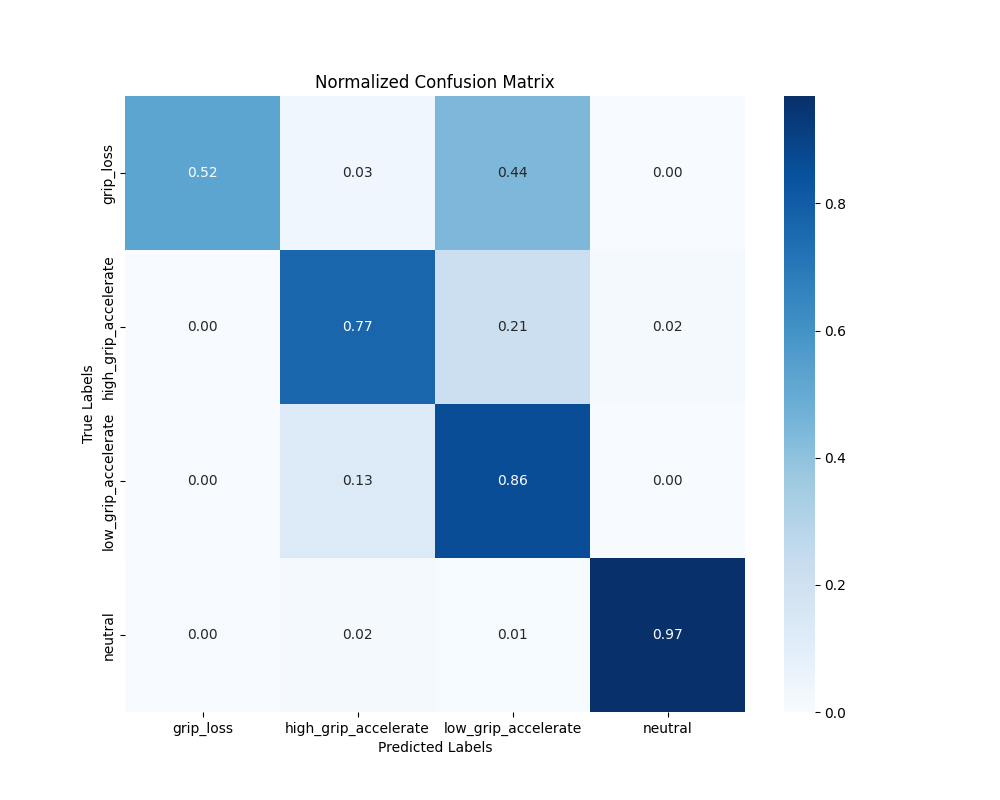
\includegraphics[width=0.55\textwidth]{img/0NO.png}
    \caption{Simple CNN normalized confusion matrix.}
    \label{fig:confusion_matrix}
\end{figure}

\begin{figure}[H]
    \centering
    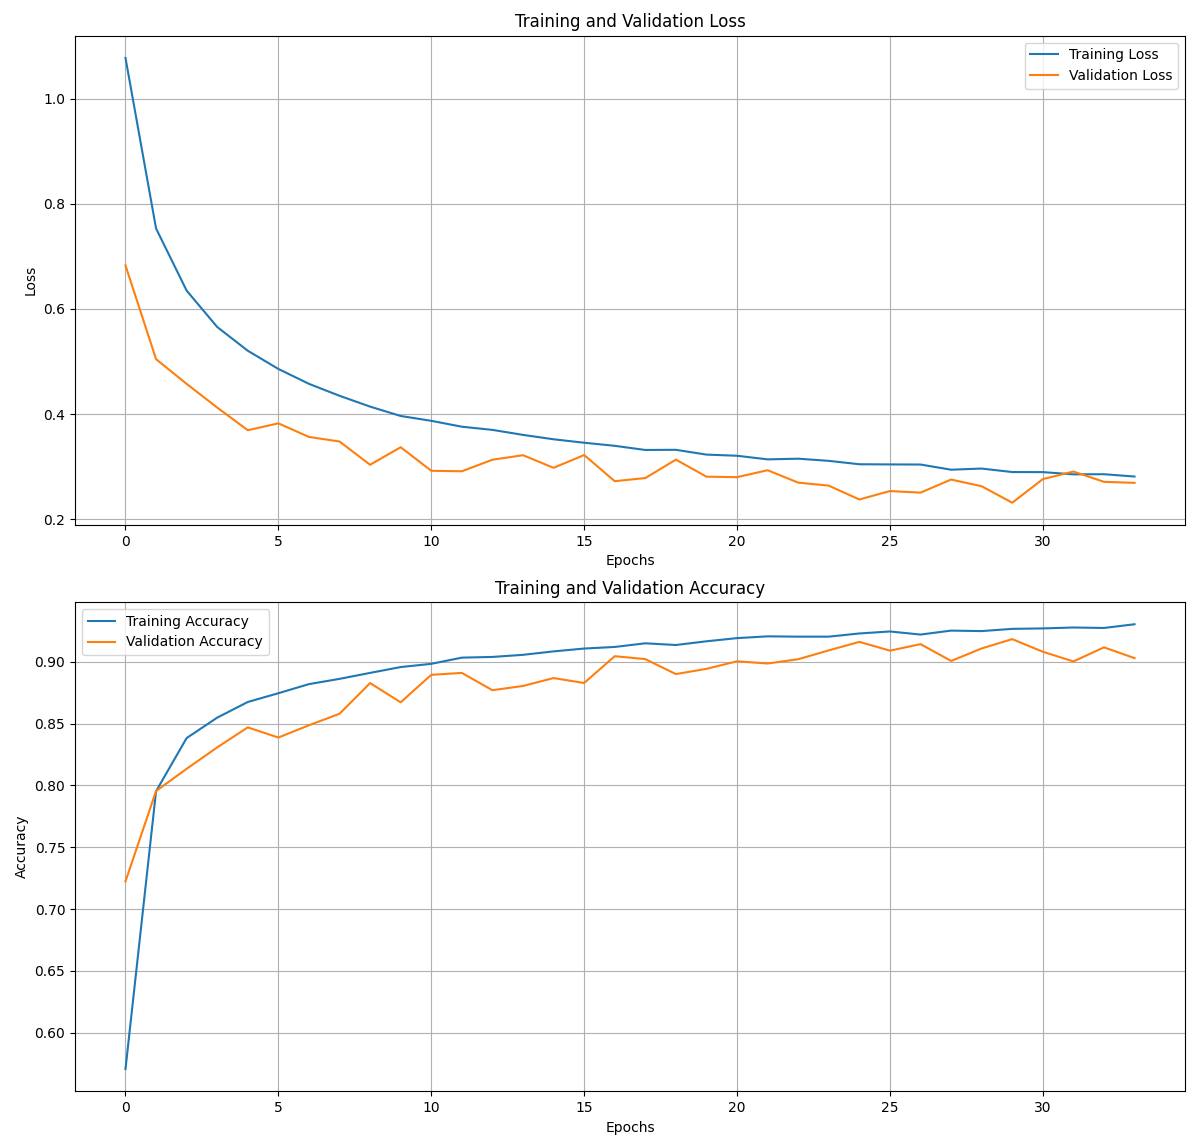
\includegraphics[width=0.55\textwidth]{img/0NOLoss.png}
    \caption{Trend of loss and accuracy during training and validation of simple CNN.}
    \label{fig:training_validation}
\end{figure}

\subsubsection{Results obtained}
The results obtained by the model on the test set are summarized below:
\begin{itemize}
    \item \textbf{Class precision:}
    \begin{itemize}
        \item \textit{grip\_loss:} 0.69
        \item \textit{high\_grip\_accelerate:} 0.84
        \item \textit{low\_grip\_accelerate:} 0.62
        \item \textit{neutral:} 1.00
    \end{itemize}
    \item \textbf{Macro Average Precision:} 0.78
    \item \textbf{Average Precision:} 0.91
\end{itemize}

These results show a good ability of the model to distinguish between different classes, with particularly high accuracy for the \textit{neutral} class. However, there is more difficulty in correctly recognizing the class \textit{low\_grip\_accelerate}, which could be improved with further optimization or data balancing techniques.

\subsection{LSTM model}
The LSTM model (\textit{Long Short-Term Memory}) is designed to exploit the sequential nature of telemetry data, taking into account temporal dependencies between samples. This approach is particularly useful for capturing the evolution of grip behavior over time, considering factors such as tire wear and driving conditions.

\subsubsection{Model Architecture}
The LSTM model consists of a sequence of layers designed to process temporal data. The structure of the model is shown below:

\begin{lstlisting}[language=Python, caption=Architecture of the LSTM model]
model = Sequential([
    Input(shape=(X_train.shape[1], X_train.shape[2])),
    LSTM(64, return_sequences=False),
    Dropout(0.3),
    Dense(64, activation='relu'),
    Dropout(0.2),
    Dense(32, activation='relu'),
    Dense(4, activation='softmax')
])
\end{lstlisting}

\begin{itemize}
    \item \textbf{Input layer:} Accepts time sequences with a length equal to \textit{window\_size = 3} and with a number of features equal to the number of numerical columns selected.
    \item \textbf{LSTM layer:} The LSTM layer with 64 units is the core of the model. This layer can store long-term and short-term information, making it ideal for capturing temporal dependencies in the data. The option \textit{return\_sequences=False} indicates that the layer returns only the final sequence output, which represents a summary of the temporal information.
    \item \textbf{Dense layers:} After the LSTM layer, the model includes two dense layers (\textit{Dense}) with 64 and 32 nodes respectively, both with ReLU activation function. These layers further process the information extracted from the LSTM layer.
    \item \textbf{Output Layer:} The final layer consists of 4 nodes with activation function \textit{softmax}, corresponding to the four grip classes to be predicted.
    \item \textbf{Dropout:} Layers of \textit{Dropout} were included with rates of 30\% and 20\% to reduce the risk of overfitting.
\end{itemize}

\subsubsection{Inclusion of Time with time index}
A key aspect of this model is the inclusion of the \textit{time\_idx} column, which represents the time index within each driving session. This field allows the model to understand that time is running and that, as a result, there will be a progressive reduction in \textit{slip} due to tire wear.\\

The column \textit{time\_idx} was calculated as follows:
\begin{lstlisting}[language=Python, caption=Calculation of \textit{time\_idx}]
df["time_idx"] = 
df.groupby(["track", "driver", "temp"]).cumcount()
\end{lstlisting}
This approach assigns an incremental index to each sample within each combination of circuit, driver, and temperature, providing the model with an explicit indication of temporal progression.

\subsubsection{Creation of Temporal Sequences}
To train the LSTM model, the data were transformed into time sequences of fixed length (\textit{window\_size}). Each sequence consists of \textit{window\_size} consecutive samples, while the label associated with the sequence corresponds to the value in the \textit{result} column of the final window sample. These samples are not mixed for the purpose of more accurate prediction. The window size length equal to 3 was decided on the fact that the time window should be neither too short in order to have only little information, nor too long because if not, the main factor of prediction in high-speed curve is lost. The code for creating the sequences is given below:

\begin{lstlisting}[language=Python, caption=
Creation of time sequences]
for name, group in df.groupby(group_cols):
    if len(group) < window_size:
        continue
    group = group.reset_index(drop=True)
    for i in range(len(group) - window_size):
        window = group.iloc[i:i + window_size]
        sequences.append(window[feature_cols].to_numpy())
        labels.append(group.iloc
                    [i + window_size - 1]["result"])
\end{lstlisting}

\subsubsection{Model evaluation}
The model was trained using the optimizer \textit{Adam} and the loss function \textit{categorical crossentropy}. During training, a \textit{early stopping} mechanism was used to stop the process when the performance on the validation set did not improve for 7 consecutive epochs.\\

The final results of the model were evaluated on the test set, with metrics such as accuracy per class and normalized confusion matrix. The inclusion of \textit{time\_idx} allowed the model to better capture temporal dynamics, improving its ability to correctly predict grip behavior as a function of time.

\subsubsection{Display of Results}.
To analyze the performance of the LSTM model, the following graphs were generated:
\begin{itemize}
    \item \textbf{Normalized confusion matrix}:   
    It can be seen that the model achieved particularly high accuracy for the \textit{neutral} class, while the other classes show a slight overlap, which could be further improved with data balancing techniques, but difficult to apply in this context.

    \item \textbf{Loss and accuracy trend:} The graphs in Figure \ref{fig:lstm_training_validation} show the evolution of \textit{loss} and \textit{accuracy} during the training and validation epochs. A gradual reduction in loss and improvement in accuracy can be observed, with stable convergence toward the end of training.
\end{itemize}

\begin{figure}[H]
    \centering
    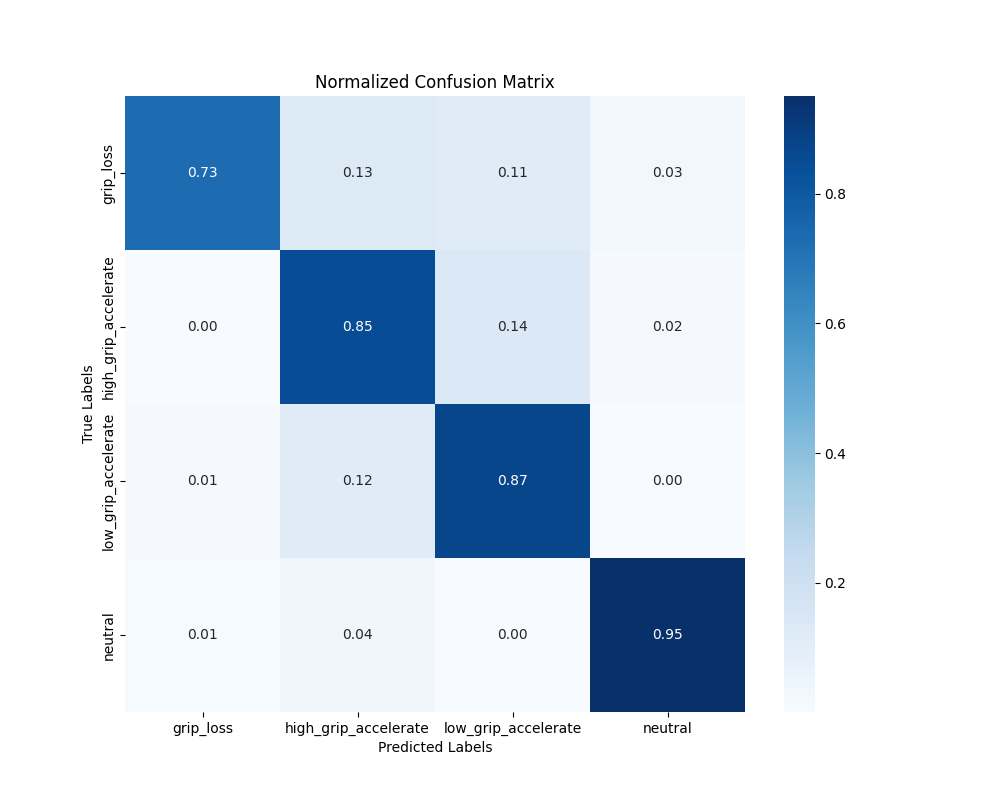
\includegraphics[width=0.55\textwidth]{img/1NO.png}
    \caption{Normalized confusion matrix of the LSTM model.}
    \label{fig:lstm_confusion_matrix}
\end{figure}

\begin{figure}[H]
    \centering
    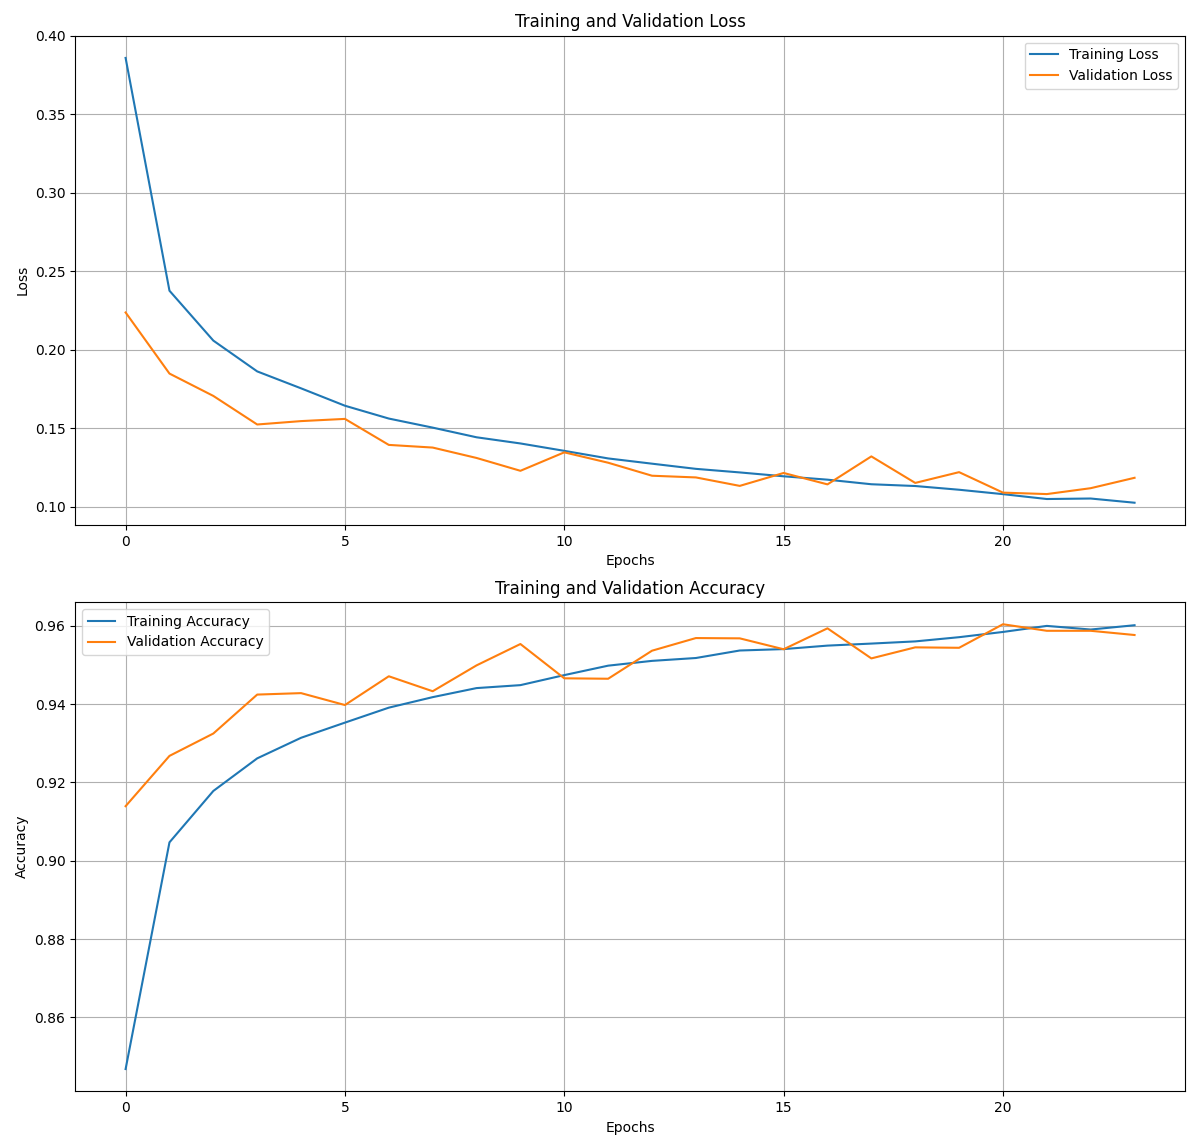
\includegraphics[width=0.55\textwidth]{img/1NOLoss.png}
    \caption{Trend of loss and accuracy during training and validation of the LSTM model.}
    \label{fig:lstm_training_validation}
\end{figure}

\subsubsection{Results obtained}.
The results obtained from the LSTM model on the test set are summarized below:
\begin{itemize}
    \item \textbf{Precision per class:}
    \begin{itemize}
        \item \textit{grip\_loss:} 0.85
        \item \textit{high\_grip\_accelerate:} 0.91
        \item \textit{low\_grip\_accelerate:} 0.82
        \item \textit{neutral:} 0.98
    \end{itemize}
    \item \textbf{Macro Average Precision:} 0.89
    \item \textbf{Average Precision:} 0.94
\end{itemize}

These results highlight that the LSTM model is one of the best among those developed because of its ability to capture temporal dependencies in the data. The high accuracy for all classes, particularly for \textit{neutral} and \textit{high\_grip\_accelerate}, demonstrates the effectiveness of the temporal sequence approach. In addition, the inclusion of the \textit{time\_idx} column allowed the model to better understand the temporal evolution of grip, further improving overall performance.


\subsection{Transformer}
The Transformer model is designed to exploit temporal relationships in telemetry data, using an architecture based on multi-headed attention mechanisms (\textit{Multi-Head Attention}). This architecture is particularly suitable for capturing long-term dependencies in sequential data, overcoming some limitations of recurrent models such as LSTM.\\

The implemented model is inspired by the example provided in the official Keras documentation \cite{keras_transformer_example} and has an optimized structure for the time sequence classification problem.

\subsubsection{Model Architecture}.
The model consists of the following main components:
\begin{itemize}
    \item \textbf{Input layer:} It accepts time sequences of fixed length (\textit{window\_size}) and with a number of features equal to that of the selected numerical columns.
    \item \textbf{Encoder Transformer:} Two Transformer encoder blocks, each consisting of:
    \begin{itemize}
        \item \textit{Multi-Head Attention:} Allows the model to focus on different parts of the sequence in parallel, capturing long-term relationships.
        \item \textit{Dropout:} Reduces the risk of overfitting.
        \item \textit{Layer Normalization:} Stabilizes training by normalizing the output.
        \item \textit{Feed-Forward Network:} A 1D convolutional network with ReLU activation to further process the information.
    \end{itemize}
    \item \textbf{Global Average Pooling:} Reduces dimensionality by aggregating information along the temporal dimension.
    \item \textbf{Dense Layers:} Two dense layers with 128 and 4 nodes respectively, used for final classification.
    \item \textbf{Batch Normalization and Dropout:} They improve training stability and reduce the risk of overfitting.
\end{itemize}

The network code is given below:
\begin{lstlisting}[language=Python, caption=Architecture of the Transformer model]
def transformer_encoder(inputs, head_size, num_heads, 
        ff_dim, dropout=0):
    x = layers.MultiHeadAttention(key_dim=head_size, 
        num_heads=num_heads, dropout=dropout)(inputs, inputs)
    x = layers.Dropout(dropout)(x)
    x = layers.LayerNormalization(epsilon=1e-6)(x + inputs)

    ff = layers.Conv1D(filters=ff_dim, kernel_size=1, 
        activation="relu")(x)
    ff = layers.Dropout(dropout)(ff)
    ff = layers.Conv1D(filters=inputs.shape[-1],
        kernel_size=1)(ff)
    return layers.LayerNormalization(epsilon=1e-6)(x + ff)

def build_model(input_shape, n_classes):
    inputs = Input(shape=input_shape)
    x = transformer_encoder(inputs, head_size=64, 
            num_heads=4, ff_dim=64, dropout=0.2)
    x = transformer_encoder(x, head_size=64, 
            num_heads=4, ff_dim=64, dropout=0.2)
    x = layers.GlobalAveragePooling1D()(x)
    x = layers.Dense(128, activation="relu")(x)
    x = layers.BatchNormalization()(x)
    x = layers.Dropout(0.3)(x)
    outputs = layers.Dense(n_classes, activation="softmax")(x)
    return Model(inputs, outputs)
\end{lstlisting}

\subsubsection{Model Parameters}
The model has a total of 61.476 parameters, of which:
\begin{itemize}
    \item \textbf{Parameters Trainable:} 61,220 (239.14 KB).
    \item \textbf{Non-Trainable parameters:} 256 (1.00 KB).
\end{itemize}
This configuration balances model complexity with computational efficiency, making it suitable for the temporal sequence classification problem.

\subsubsection{Transformer Operation}
The Transformer uses the attention mechanism to assign different weight to each element in the sequence, based on its relevance to the classification task. This approach allows the model to capture complex relationships among the data, even when temporal dependencies span long sequences.\\

The use of \textit{Global Average Pooling} reduces the dimensionality of sequences by aggregating the most relevant information along the temporal dimension. The final dense layers process this information to produce the final classification.

\subsubsection{Use of Time Index and Early Stopping}
The time index \textit{time\_idx} was also used in the Transformer model to indicate the temporal progression within driving sessions. This approach allowed the model to capture the temporal evolution of grip, taking into account factors such as tire wear and driving conditions. In addition, the \textit{Custom Early Stopping} mechanism, described above, was implemented.

\subsubsection{Display of Results}
To analyze the performance of the Transformer model, the following graphs were generated:

\begin{itemize}
    \item \textbf{Normalized Confusion Matrix:}  
    The normalized confusion matrix, shown in Figure \ref{fig:transformer_confusion_matrix}, shows that the model performed well for the class \textit{neutral}, with very high accuracy. However, there is significant overlap for the class \textit{grip\_loss}, which is more difficult to distinguish than the others. This suggests that the Transformer model, while effective, does not achieve the performance of the LSTM model for some classes.

    \item \textbf{Loss and accuracy trend:}  
    The graphs in Figure \ref{fig:transformer_training_validation} show the evolution of loss (\textit{loss}) and accuracy (\textit{accuracy}) during the training and validation epochs. A gradual reduction in loss and improvement in accuracy is observed, with stable convergence toward the end of training. However, fluctuations in the validation curve indicate that the model is affected by weight class balancing.
\end{itemize}

\begin{figure}[H]
    \centering
    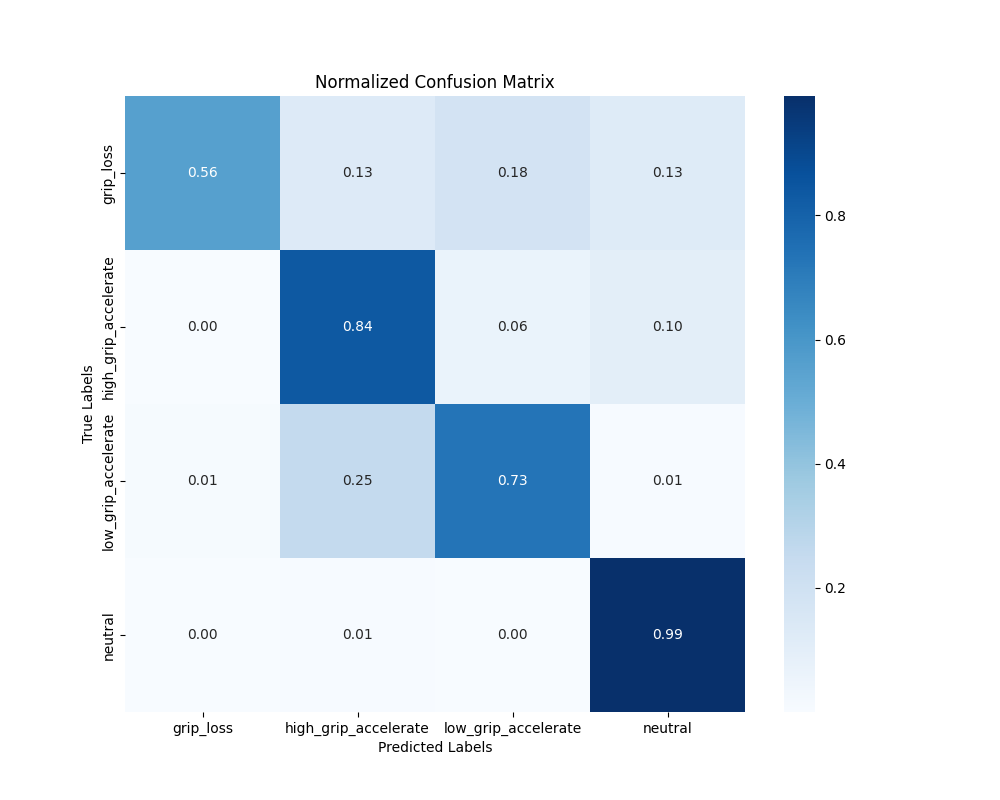
\includegraphics[width=0.8\textwidth]{img/2Sì.png}
    \caption{Normalized confusion matrix of the Transformer model.}
    \label{fig:transformer_confusion_matrix}
\end{figure}

\begin{figure}[H]
    \centering
    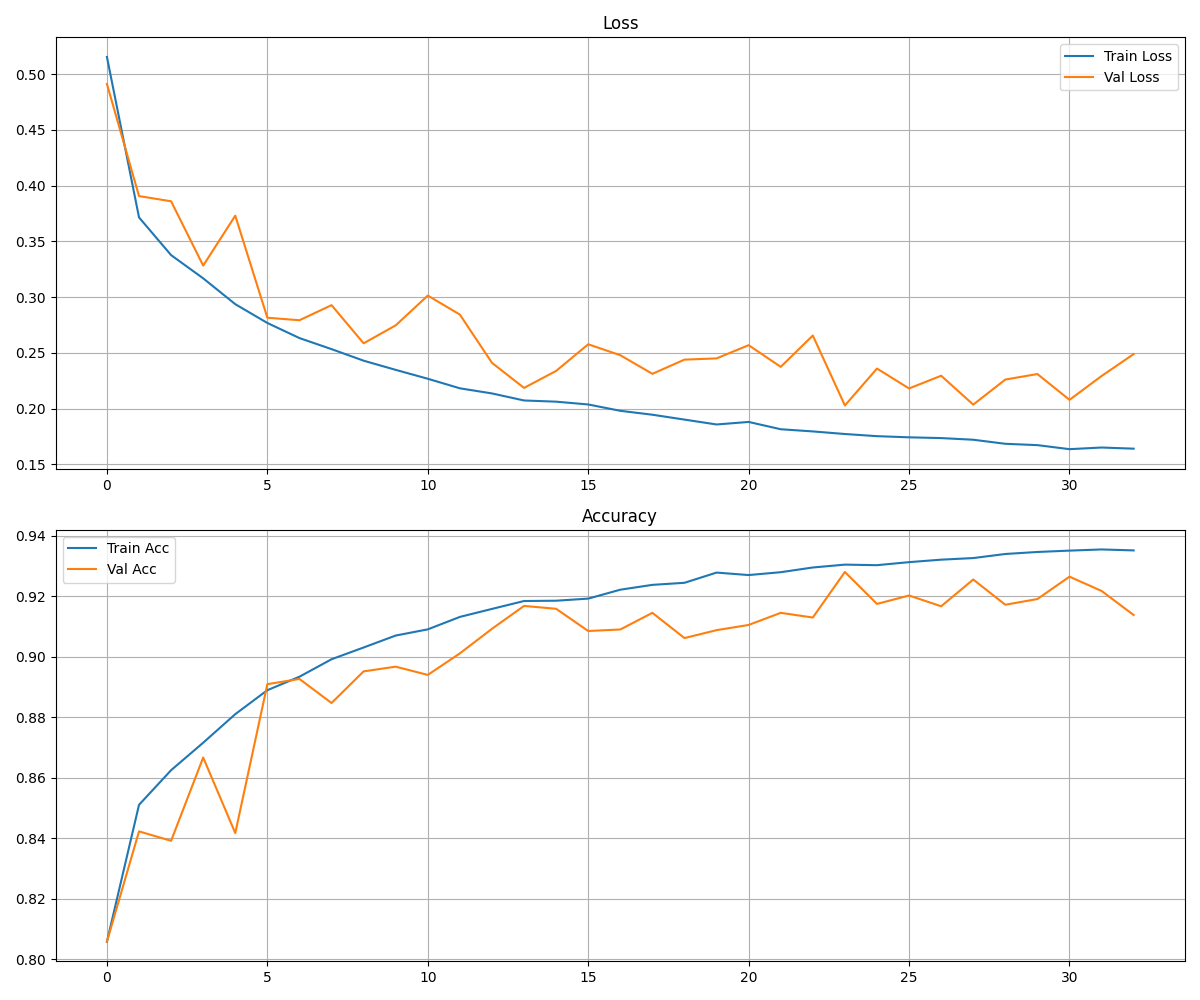
\includegraphics[width=0.8\textwidth]{img/2SìLoss.png}
    \caption{Trend of loss and accuracy during training and validation of the Transformer model.}
    \label{fig:transformer_training_validation}
\end{figure}

\subsubsection{Achievements}
The results obtained from the Transformer model on the test set are summarized below:
\begin{itemize}
    \item \textbf{Precision per class:}
    \begin{itemize}
        \item \textit{grip\_loss:} 0.58
        \item \textit{high\_grip\_accelerate:} 0.87
        \item \textit{low\_grip\_accelerate:} 0.72
        \item \textit{neutral:} 0.98
    \end{itemize}
    \item \textbf{Macro Average Precision:} 0.79
    \item \textbf{Average Precision:} 0.91
\end{itemize}

These results show that the Transformer model is able to achieve good overall performance, with high accuracy for the \textit{neutral} class and acceptable results for the other classes. However, its performance is not comparable to that of the LSTM model, particularly for the \textit{grip\_loss} class, which has lower accuracy. However, the inclusion of the \textit{time\_idx} column allowed the model to capture temporal dependencies, improving prediction ability compared to a static approach.

\subsection{ResNet 1D Model for Tabular Data}
The ResNet 1D model is designed to exploit the capabilities of ResNet networks (\textit{Residual Networks}) applied to tabular data. This approach differs from other models used in that it introduces residual blocks, which allow for improved gradient propagation during training and for dealing with vanishing gradient problems, which are particularly relevant in deep networks.

\subsubsection{Network Architecture}
The implemented ResNet 1D network consists of a sequence of residual blocks designed to process tabular data. Each residual block consists of:
\begin{itemize}
    \item \textbf{Linear layers:} Two linear layers with constant size (128 nodes) within each residual block.
    \item \textbf{Batch Normalization:} Stabilizes training by normalizing the output of each linear layer.
    \item \textbf{ReLU Activation:} Introduces nonlinearities to improve the learning capability of the network.
    \item \textbf{Remaining connections:} Allows the original block input to be summed to the processed output, facilitating gradient propagation and improving the learning ability of the network.
\end{itemize}

The architecture of the model is as follows:
\begin{itemize}
    \item \textbf{Input layer:} A linear layer that projects input data into a 128-dimensional space, followed by a ReLU activation function and batch normalization.
    \item \textbf{Residual Blocks:} A sequence of residual blocks (the number is determined by the parameter \textit{depth}, set to 3 in the provided model).
    \item \textbf{Output Layer:} A linear layer that reduces the size from 128 to 64, followed by a ReLU activation function and an additional linear layer that maps the 64 nodes to the output nodes corresponding to the number of classes.
\end{itemize}

\subsubsection{Advantages of the ResNet 1D Model}
The use of a ResNet 1D network for tabular data offers several advantages over traditional approaches:
\begin{itemize}
    \item \textbf{Gradient Propagation:} Residual connections facilitate gradient propagation during training, reducing the risk of vanishing gradient.
    \item \textbf{Generalization Capability:} Residual blocks allow the network to learn deeper and more complex representations, improving generalization ability.
    \item \textbf{Adaptability to Tabular Data:} The use of linear layers and residual connections enables the capture of complex patterns in tabular data, making the model particularly suitable for classification problems.
\end{itemize}

\subsubsection{Model Implementation}.
The model was implemented in PyTorch and has the following structure:
\begin{lstlisting}[language=Python, caption=Architecture of the ResNet 1D model]
class ResidualBlock(nn.Module):
    def __init__(self, dim):
        super().__init__()
        self.block = nn.Sequential(
            nn.Linear(dim, dim),
            nn.BatchNorm1d(dim),
            nn.ReLU(),
            nn.Linear(dim, dim),
            nn.BatchNorm1d(dim)
        )

    def forward(self, x):
        return F.relu(x + self.block(x))

class ResNet1DTabular(nn.Module):
    def __init__(self, input_dim, num_classes, depth=3):
        super().__init__()
        self.input_layer = nn.Sequential(
            nn.Linear(input_dim, 128),
            nn.ReLU(),
            nn.BatchNorm1d(128)
        )
        self.res_blocks = nn.Sequential(*[ResidualBlock(128) 
            for _ in range(depth)])
        self.output_layer = nn.Sequential(
            nn.Linear(128, 64),
            nn.ReLU(),
            nn.Linear(64, num_classes)
        )

    def forward(self, x):
        x = self.input_layer(x)
        x = self.res_blocks(x)
        return self.output_layer(x)
\end{lstlisting}

\subsubsection{Use of Temporal Index and Early Stopping}
The temporal index \textit{time\_idx} was also used in this model to indicate the temporal progression within driving sessions. This approach allowed the model to capture the temporal evolution of grip, taking into account factors such as tire wear and driving conditions.
In addition, the \textit{Custom Early Stopping} mechanism described above was implemented.

\subsubsection{Display of Results}
To analyze the performance of the ResNet 1D model, the following graphs were generated:

\begin{itemize}
    \item \textbf{Normalized Confusion Matrix:}  
    The normalized confusion matrix, shown in Figure \ref{fig:resnet_confusion_matrix}, shows that the model performed well overall.

    \item \textbf{Loss and accuracy trend:}  
    The graphs in Figure \ref{fig:resnet_training_validation} show the evolution of loss (\textit{loss}) and accuracy (\textit{accuracy}) during the training and validation epochs.
\end{itemize}

\begin{figure}[H]
    \centering
    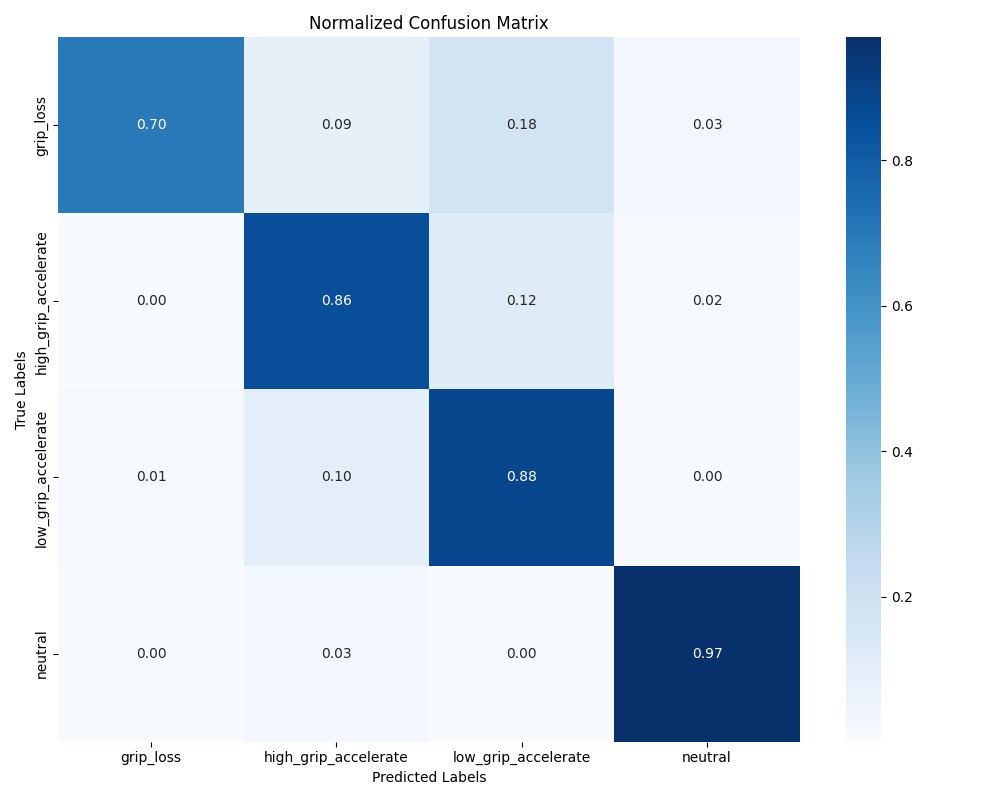
\includegraphics[width=0.8\textwidth]{img/3Sì.png}
    \caption{Normalized confusion matrix of the ResNet 1D model.}
    \label{fig:resnet_confusion_matrix}
\end{figure}

\begin{figure}[H]
    \centering
    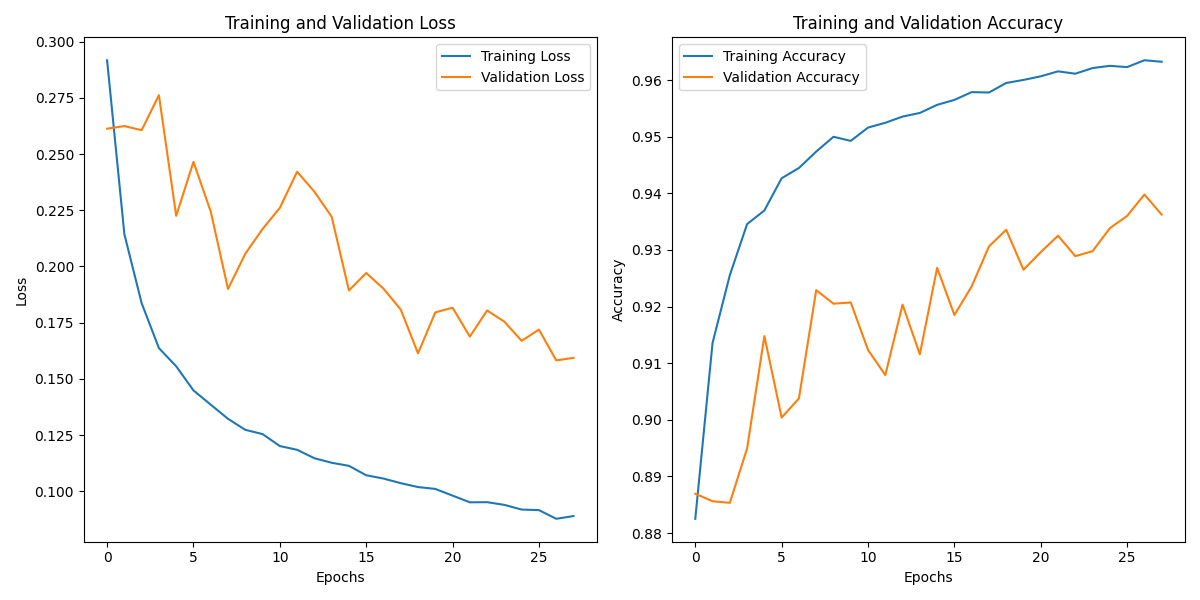
\includegraphics[width=0.8\textwidth]{img/3SìLoss.png}
    \caption{
Trend of loss and accuracy during training and validation of the ResNet 1D model.}
    \label{fig:resnet_training_validation}
\end{figure}

\subsubsection{Results obtained}.
The results obtained from the ResNet 1D model on the test set are summarized below:
\begin{itemize}
    \item \textbf{Precision per class:}
    \begin{itemize}
        \item \textit{grip\_loss:} 0.85
        \item \textit{high\_grip\_accelerate:} 0.90
        \item \textit{low\_grip\_accelerate:} 0.81
        \item \textit{neutral:} 0.99
    \end{itemize}
    \item \textbf{Macro Average Precision:} 0.89
    \item \textbf{Average Precision:} 0.94
\end{itemize}


The ResNet 1D model achieved an overall accuracy of 94\% on the test set, with particularly high precision for the \textit{neutral} class. However, the \textit{grip\_loss} class has a lower recall (0.63), highlighting a difficulty in correctly distinguishing this class from the others. This result is influenced by the imbalance of the dataset, where the class \textit{grip\_loss} is significantly less represented than the others.

\subsubsection{Analysis}
The ResNet 1D model, along with the LSTM model, is one of the best of those tested because of its ability to capture complex patterns in temporal data. The use of residual blocks allowed the model to learn deep representations and to generalize well on test data. Despite the difficulties associated with class imbalance, the model demonstrated high overall accuracy, making it a viable choice for telemetry classification applications.

\subsubsection{Sequential Version of ResNet 1D}
In addition to the tabular version of the ResNet 1D, a variant considering a sequence of 3 elements as input was implemented in order to test whether the results could improve and become comparable to those obtained with the LSTM model. However, the results were worse than the tabular version and the LSTM.

\paragraph{Differences in Structure}
The main difference from the tabular version is the use of 1D convolutions to process time sequences. Specifically:
\begin{itemize}
    \item \textbf{1D convolutions:} The network uses 1D convolutional layers to capture local patterns in temporal sequences. Each residual block consists of two 1D convolutions with kernel size 3, followed by batch normalization and residual connections.
    \item \textbf{Pooling:} The network includes a layer of \textit{MaxPooling} to reduce dimensionality along the temporal dimension.
    \item \textbf{Output Layer:} After the residual blocks, the network uses a \textit{Adaptive Average Pooling} to aggregate the information along the temporal dimension, followed by a linear layer for final classification.
\end{itemize}

\paragraph{Reasons for Worst Results}
The worst results compared with LSTM and the tabular version of ResNet 1D can be attributed to several factors:
\begin{itemize}
    \item \textbf{Inadequacy of Structure}. Sequential ResNet 1D may not be optimal for capturing long-term temporal dependencies, which are instead well handled by LSTM models due to their ability to store long-term information.
    \item \textbf{Limited Overlap:} 1D convolutions, while effective for local patterns, may not be able to capture more complex relationships between sequence elements.
\end{itemize}

Despite the introduction of 1D convolutions and residual blocks, the sequential version of ResNet 1D did not achieve the desired performance. This result highlights that, for sequential classification problems with complex temporal dependencies, models such as the LSTM remain a more suitable choice than a ResNet designed for tabular data or short sequences.

\subsection{CNN Network With Data Augmentation}
In addition to the tests described so far, an additional possibility was tested: the idea of losing the concept of temporal sequence and not keeping the data in sequential order. In this approach, the data were divided into training and validation sets using two circuits, while a third circuit was used as a test set. This method allowed the model to be evaluated in a context where the test data came from a completely different circuit than those used for training.

\subsubsection{Model Architecture}
The model used is a fully connected neural network (CNN) with a simple structure designed to be suitable for real time predictions. The architecture consists of:
\begin{itemize}
    \item \textbf{Dense Layers:} Four fully connected layers with decreasing size (256, 128, 64, 32 nodes), each followed by a ReLU activation function.
    \item \textbf{Batch Normalization:} Applied after each dense layer to stabilize training.
    \item \textbf{Dropout:} Used to reduce the risk of overfitting, with dropout rates varying between 20\% and 30\%.
    \item \textbf{Output Layer:} A final layer with 4 nodes and softmax activation function for grip class classification.
\end{itemize}

\subsubsection{Data Augmentation}
To address class imbalance, a data augmentation technique was applied. The least represented classes were replicated until a similar number of examples were reached as the most represented class. This process improved the distribution of classes in the training set, making the model more robust.

\subsubsection{Results and Considerations}
The model performed very well on the test track (\textit{Mugello}), with an overall accuracy of 95\%. The main results are summarized below:
\begin{itemize}
    \item \textbf{Precision per class:}
    \begin{itemize}
        \item \textit{grip\_loss:} 0.84
        \item \textit{high\_grip\_accelerate:} 0.94
        \item \textit{low\_grip\_accelerate:} 0.75
        \item \textit{neutral:} 0.99
    \end{itemize}
    \item \textbf{Macro Average Precision:} 0.88
    \item \textbf{Average Precision:} 0.95
\end{itemize}

The graphs in Figure \ref{fig:cnn_training_validation} show the trends of loss (\textit{loss}) and accuracy (\textit{accuracy}) during the training and validation epochs. It is observed that the accuracy on the validation set is higher than on the training set, a behavior attributable to the use of \textit{Dropout}, which reduces overfitting during training. The loss curve stabilizes toward the end of training, indicating good model convergence.
The normalized confusion matrix, shown in Figure \ref{fig:cnn_confusion_matrix}, indicates that the model performed exceptionally well for the class \textit{neutral} (accuracy 0.99) and \textit{high\_grip\_accelerate} (accuracy 0.94). However, the class \textit{low\_grip\_accelerate} exhibits a lower accuracy (0.75), suggesting that the model may face challenges in distinguishing this class in certain cases. Nevertheless, the performance for this class is higher compared to other models, particularly for the most challenging case of \textit{grip\_loss}, where this model achieves the best recall and precision among all the models tested.\\

Despite the good performance, it is important to point out some limitations:
\begin{itemize}
    \item \textbf{Dataset labeling:} Accuracy could be affected by the fact that dataset labeling is not perfectly accurate. Improvement in the labeling process could lead to more reliable results.
    \item \textbf{Simulated Data:} The data used come from a simulator, which could limit the generalizability of the model to real data collected on a physical circuit.
    \item \textbf{Loss of Sequence Concept:} The elimination of the temporal sequence concept may have simplified the problem, but it also reduced the model's ability to capture complex temporal dependencies that might be relevant to the non-simulation-mode task.
\end{itemize}

\begin{figure}[H]
    \centering
    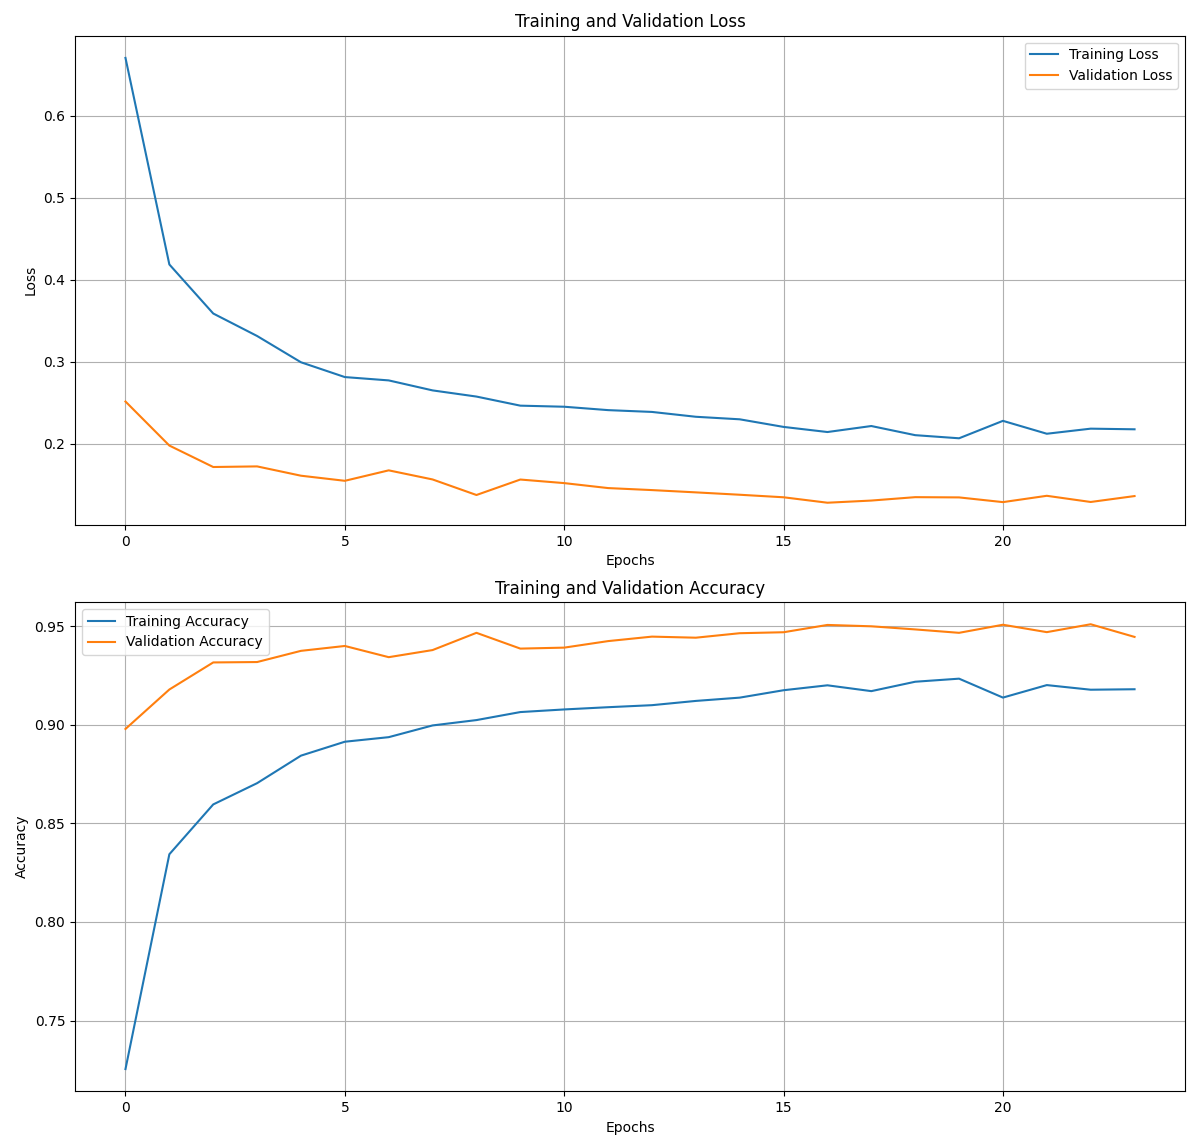
\includegraphics[width=0.6\textwidth]{img/0RandomLossSI.png}
    \caption{Trend of loss and accuracy during training and validation of the CNN model.}
    \label{fig:cnn_training_validation}
\end{figure}

\begin{figure}[H]
    \centering
    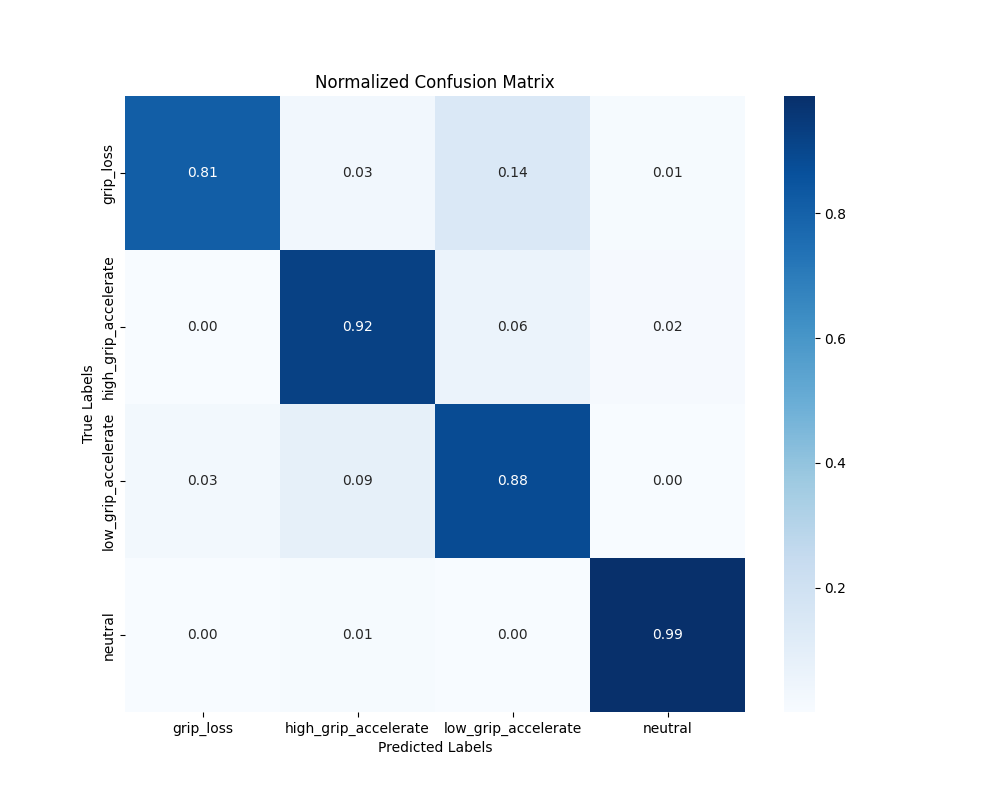
\includegraphics[width=0.6\textwidth]{img/0RandomNO.png}
    \caption{Normalized confusion matrix of the CNN model on the test circuit (\textit{Mugello}).}
    \label{fig:cnn_confusion_matrix}
\end{figure}

\subsubsection{Conclusion}
This approach has shown that very good performance can be achieved even with a simple model and without considering the temporal sequence. However, for real applications, it would be necessary to use data collected in a physical context and improve the labeling process. In addition, the use of models that consider temporal sequence, such as LSTM, could provide more robust results in more complex scenarios.

\subsection{Batch size choice}.
In the context of this work, a high \textbf{batch size} (equal to 1024) was adopted over commonly used values (e.g., 32 or 64). This choice is motivated by the \textbf{balanced nature of the dataset}, in which the neutral class is largely predominant.

Using a larger batch size reduces the probability that a single batch will contain only samples belonging to the majority class, thus improving the representativeness of minority classes during training. In addition, this strategy was particularly useful in combination with \textbf{weighting of class weights}, which was applied to further compensate for the imbalance. In summary, the choice of a batch size of 1024 helped to make the learning process more effective by ensuring better generalization of the model over the less frequent classes.

\section{Future Grip Classification with Machine Learning}

\section{Front and Back Slip Regression with Machine Learning}


\newpage

\section{User Interface}
The user interface is designed to provide clear and immediate visual support while driving, showing in real time the behavior of the tires and the type of grip detected by the predictive model. The goal is to make grip dynamics understandable even to non-expert users by intuitively highlighting which wheels are losing grip and what overall behavior the car has at that moment.

\subsection{Requirements}

\subsubsection{Functional requirements}
The functional requirements of the interface are:
\begin{itemize}
    \item Schematic visualization of the car as seen from above with the four wheels represented graphically.

    \item  Each wheel must:\\
    - Show the slip (slip) value in real time.\\
    - Change color according to the slip value, according to a color scale.\\
    - Show the overall behavior of the vehicle by the label predicted by the model (e.g., grip loss, neutral, high grip accelerate, low grip accelerate).\\
    - Allow changing the predictive model to be used (selecting it from those described in the previous chapters).\\
    - Real-time synchronization with data provided by the simulator (Assetto Corsa).
\end{itemize}

\subsubsection{Non-functional requirements}
The nonfunctional requirements of the interface are:

\begin{itemize}
    \item \textbf{Responsiveness:} the interface must update frequently enough to make the evolution of the slip and predicted labels smooth and understandable (at least 10 FPS).
    \item \textbf{Usability:} the interface must be simple, intuitive, and accessible even to users who are not technical experts.
    \item \textbf{Compatibility:} it must be compatible with the main operating systems (Windows, Linux) and easily integrated with the data stream coming from Assetto Corsa.
    \item \textbf{Extendability:} the interface must be modularly designed to allow future addition of new features, such as multiple session analysis or model comparison.
    \item \textbf{Performance:} the interface must not introduce significant delays in data flow or in rendering the driving experience.
\end{itemize}

\subsection{Design}
The design phase of the user interface was guided by two main objectives: first, the clarity and intuitiveness of the real time visualization of wheel behavior, and second, the ability to return concise but meaningful information to the user regarding the overall state of the vehicle while driving.\\
The interface design was conceived to adapt to a dynamic context such as a real-time driving simulation, where the user (driver or developer) cannot devote prolonged attention to data analysis but needs instantaneous, intuitive, visually coded information.\\

The interface is divided into two main areas:
\begin{itemize}
    \item \textbf{Wheel View:} stylized representation of the car as seen from above with four wheels. Each wheel shows a numeric slip indicator and changes color according to its value. This section provides an immediate readout of tire condition and any localized slip.
    \item \textbf{Overall status indicator:} a section dedicated to displaying the label predicted by the currently active AI model. The label is shown both textually and with an associated color and possibly an icon. The goal is to provide the driver or user with a summary of the vehicle's overall grip.
\end{itemize}

Graphic choices were geared toward maximizing contrast and readability, using a color palette suitable for low visual concentration situations.

\subsubsection{Personas and scenarios}
To properly define the needs of the interface users, three representative profiles (personas) were created, each with different needs and skill levels. A typical usage scenario was defined for each person.
\begin{itemize}
    \item \textbf{Person 1:} \\
    - Name: Luke\\
    - Role: Advanced Sim Racer\\
    - Age: 24 years old\\
    - Profession: Mechanical engineering student\\
    - Experience: High, has been using Assetto Corsa for years\\
    - Goal: Improve cornering performance by optimizing grip management\\
    - Scenario: Luca uses the interface during free practice on a technical circuit to analyze the moments when the front tires start to slip. Using the slip visualization and the label predicted by the model, he can tell if he can still accelerate or if he has reached the limit.
    \item \textbf{Person 2:}\\
    - Name: Julia\\ 
    - Role: Junior AI engineer in motorsport\\
    - Age: 27 years old\\
    - Profession: Data scientist in a startup\\
    - Experience: Medium in racing, high in machine learning\\
    - Goal: Validate model predictions in realistic context\\
    - Scenario: Julia uses the interface to observe the behavior of the classifier in real time, comparing the model output with real slip values to evaluate the accuracy of the network. She needs a clear interface for A/B testing between different models.
    \item \textbf{Person 3:}\\
    - Name: Matthew\\ 
    - Role: Technical viewer at an event\\
    - Age: 35 years old\\
    - Profession: Motorsports enthusiast, but not technical expert\\
    - Experience: Low\\
    - Goal: To better understand what happens during the race\\
    - Scenario: Matthew attends an event where the on-screen interface is shown. He immediately understands which wheels are losing grip because of the color, and he grasps the importance of the car's behavior because of the visual label. The interface helps him interpret driving even without knowing the raw data.
\end{itemize}

\subsubsection{Focus Group}
To validate the design choices and gather qualitative feedback, a focus group was organized with 6 participants, divided equally between experienced users (sim racers, engineering students) and non-technical users (motor enthusiasts and outside observers). The meeting was structured in three phases:

\begin{itemize}
    \item \textbf{Display:} a prototype of the interface (mockup or static simulation) was shown with a short video showing the evolution of the slip during a lap on a track.
    \item \textbf{Interaction:} users tried to interact with the interface, simulating a real time test (using pre-recorded data).
    \item \textbf{Discussion:} an open, question-driven feedback gathering session was conducted.
\end{itemize}
Main observations gathered:
\begin{itemize}
    \item Technical users appreciated the ability to see the precise numerical value of the slip, and also asked about the ability to customize color thresholds.
    \item Non-technical users found the color code and overall label very useful, but suggested adding icons or symbols to make it easier to understand at a glance.
    \item Some participants suggested substitute with a brief explanatory text each label (e.g., “you can speed up again,” “you are on the limit,” “you have lost grip”).
\end{itemize}

The interface concept was found to be positive and useful by all participants. The proposals that emerged will be taken into consideration in subsequent iterations, particularly to improve the visual accessibility and readability of information by users with different levels of experience.

\subsubsection{Interface design}
With regard to user interface design, it focused on a number of fundamental principles geared toward usability and adaptability to ensure a smooth and effective user experience, even in a dynamic context such as driving simulation.\\

The main aspects considered are:
\begin{itemize}
    \item \textbf{Accessibility by design:} the interface was designed with accessibility principles in mind from the initial stages. A high color contrast was chosen to ensure readability even in low light conditions or for users with visual impairments (such as color blindness). All visual elements were designed to be perceivable without ambiguity, and text labels accompany colors to avoid interpretative ambiguities.
    \item \textbf{Responsive layout:} the interface layout automatically adapts to the size and resolution of the device in use, whether it is a desktop monitor, a tablet, or a second dedicated screen in the simulator location. Elements are rearranged to optimize readability and interaction in any context, without loss of information.
\end{itemize}

In line with user-centered design best practices, the interface design phase was accompanied by the creation of static mockup, which were useful for validating the positioning of elements, color choices, and information flow.

\begin{figure}[H]
\centering
\includegraphics[width=0.7\textwidth]{img/mockup.png}
\caption{Graphical mockup of the application interfaces.}
\label{fig:mockup}
\end{figure}


The mockup above \ref{fig:mockup} shows the basic structure of the interface: in the center, there is an image that represents the silhouette of the car with the four wheels, each colored according to the real time slip value and accompanied by a numerical value. At the bottom is the global state label predicted by the AI model, and at the top, a Combo Box to select the Machine learning model.

\subsection{User Interaction}
Interaction with the interface is not limited to the visual aspect, but is designed to provide a multimodal experience, also taking advantage of sound and potentially haptic signals to provide real-time feedback to the user while driving.

\begin{itemize}
    \item \textbf{Visual Interaction:} the user can easily monitor wheel status through intuitive color coding and numerical values updated in real time. The overall label provides a clear summary of the vehicle's status, proving especially useful at critical times, such as during cornering or challenging driving situations.
    \item \textbf{Sound Interaction:} an audible notification system has been designed to provide immediate feedback to the driver:
    \begin{itemize}
        \item A simple sound signal \cite{bip_sound} to indicate a high grip state.
        \item A higher-pitched signal \cite{bip_sound_machine} to warn that you are at the limit of the model's intended grip.
        \item An error sound signal \cite{beep_warning} to notify you of loss of grip during the course.
    \end{itemize}
\end{itemize}

\subsection{Technology}
The application was developed using the Python programming language and the PyQt5 library, one of the most powerful libraries for creating cross-platform graphical user interfaces. PyQt5 offers a wide range of tools for designing modern, interactive GUIs, allowing the integration of advanced features such as event handling, graphical rendering, and multimedia support.

\subsubsection{Application Technology Structure}
The application consists of several main components:
\begin{itemize}
    \item \textbf{WheelVisualizer:} a custom widget that uses the \texttt{QPainter} module to draw a graphical representation of the vehicle wheels. Each wheel is dynamically colored according to the slip value, which is calculated and updated in real time.
    \item \textbf{MainWindow:} the main window of the application, which includes:
    \begin{itemize}
        \item A model selector (\texttt{QComboBox}) for choosing between different prediction algorithms.
        \item A status label (\texttt{QLabel}) showing summary information about the vehicle status.
        \item A sound notification system (\texttt{QSoundEffect}) to provide immediate feedback to the driver based on the predicted state.
    \end{itemize}
\end{itemize}

\subsubsection{Technologies Used}
\begin{itemize}
    \item \textbf{PyQt5:} used for creating the graphical user interface, including custom widgets, event management, and graphical rendering.
    \item \textbf{QPainter:} employed for wheel and vehicle body design, with a responsive design that adapts to the window size.
    \item \textbf{QSoundEffect:} used to implement a sound notification system that alerts the user in real time.
    \item \textbf{QTimer:} used to periodically update wheel slip and vehicle status data.
\end{itemize}

\subsubsection{Data Exposure via WebSocket}
Data processed by the application are made available in real time through a WebSocket connection.
This allows for:
\begin{itemize}
    \item Receive slip, and classification information asynchronously;
    \item Integrate the results into a Web interface or any client compatible with the WebSocket protocol;
    \item Dynamically update graphs and visualizations without reloading the page or interrupting program execution.
\end{itemize} 

\subsection{Testing}
\subsubsection{User interface evaluation with the UEQ questionnaire}

To assess the quality of the graphical user interface of the application \textit{Slip Dashboard}, the User Experience Questionnaire (UEQ) was administered to a sample of 10 users. The questionnaire consists of 26 pairs of opposing adjectives, grouped into six main categories reflecting different dimensions of user experience:
\begin{itemize}
    \item \textbf{Attractiveness}: Overall rating of interface enjoyment.
    \item \textbf{Clearness/Learnability}: How easy the interface is to understand and learn.
    \item \textbf{Efficiency}: How quickly the interface allows operations to be performed.
    \item \textbf{Controllability}: Feeling of control by the user.
    \item \textbf{Stimulation}: How interesting and engaging the interface is.
    \item \textbf{Originality}: Perception of innovation and creativity.
\end{itemize}

Each item is rated on a 7-point scale where the extremes represent the two opposite characteristics (e.g., “annoying” vs. “pleasant,” "neat" vs. “overloaded”).\\
The interface under consideration (Fig.\ref{fig:GUI}) was tested in simulated mode, and the data were processed according to the methodological directions of the UEQ manual. The results were analyzed in terms of:
\begin{itemize}
    \item Overall and single dimension mean and standard deviation.
    \item Statistical accuracy by 95 percent confidence interval for each scale.
    \item Display of distribution of responses by item and by group.
    \item Internal consistency of groups (checked by Cronbach's $\alpha$ coefficient).
\end{itemize}
Overall, the simulated results showed a positive evaluation, particularly for the scales \textit{Efficiency} and \textit{Learnability}, while dimensions such as \textit{Originality} and \textit{Stimulation} scored slightly lower but still in the positive area.\\
This evaluation represents a first step toward optimizing the interface, providing concrete indications of what graphical or functional aspects can be further improved in future versions.

\newpage
\subsection{Final Result}
The end result is an intuitive and functional Graphical User Interface designed to monitor in real time and provide immediate feedback to the driver. The interface is shown in the figure \ref{fig:GUI}.
\begin{figure}[H]
\centering
\includegraphics[width=1\textwidth]{img/gui.PNG}
\caption{The application interface.}
\label{fig:GUI}
\end{figure}

\chapter{Future Developments}
The present work represents only the first step in a vast and evolving field of research. The potential for extension of the described system is manifold and lends itself to different areas of application, both in the context of automotive competition and in everyday mobility.

\section{Integration with Reinforcement Learning algorithms}
One of the most natural and promising developments in this study is the integration of the predictive model within the reward function of an agent based on Reinforcement Learning. Specifically, the information provided by the classifier (i.e., whether the vehicle can accelerate further into a curve, whether it has reached the limit, or whether it has lost grip) could be used as a direct penalty or incentive in the agent's learning of optimal behavior.\\

In simulative contexts such as Assetto Corsa, where autonomous driving projects based on reinforcement learning are already in place, the introduction of a reward function informed by the state of grip could significantly improve the learned driving strategy, making it more realistic and conservative at critical points on the track (curves, chicanes, changes in slope).

\section{Training on real data}
Another important future development is to train the model on data from real vehicles. Currently, the neural networks have been trained using simulated data obtained from the Assetto Corsa software; although this data is physically consistent and sufficiently complex, the introduction of datasets acquired from real cars on the track would allow an increase in the level of generalization and robustness of the model against real noise, sensor imperfections, and external variability.\\
This transition from simulated data to real data is critical to make the system usable in practical applications such as advanced driver assistance or validation of control strategies for racing vehicles.

\section{Application to the civil automotive sector}

A particularly interesting development, which opens up scenarios for applied research in the world of mobility, concerns the extension of the model to the context of road cars. With appropriate modifications and simplifications, the system could be integrated as an auxiliary module in active safety systems such as the Electronic Stability Program (ESP), providing predictive grip analysis available in real time.\\
In particular, the system could offer an additional layer of interpretation of data already acquired from on-board sensors (such as ABS, skid sensors, IMU, etc.), anticipating situations of loss of vehicle control and enabling proactive interventions.

\section{Extension to varying environmental and mechanical conditions}

To increase the generalization of the model, further future development is to introduce more diverse environmental and mechanical variables during training. Environmental temperature variability has already been considered in this work, but the model could be extended further to include:

\begin{itemize}
    \item Different weather conditions: rain, wet runway, fog or frost;
    \item Different types of tires: soft, medium, hard, intermediate or rain compounds;
    \item Different mechanical setups of the car: initial tire pressure, setup settings, aerodynamics;
    \item Types of tracks: city, street or kart tracks.
\end{itemize}

These extensions would significantly increase the model's ability to adapt to unforeseen or unseen scenarios during training, making it more suitable for integration into real-world driving contexts or advanced driver training simulators.

\section{Intelligent User Interfaces and Multichannel Feedback}
Finally, another line of development concerns the improvement of user interfaces and data visualization systems. The currently proposed interface could be enriched with vibration capabilities or voice prompts, enabling more effective multimodal interaction, especially in simulated or real-world driving contexts where visual distraction needs to be minimized.


\chapter{Conclusion}




\bibliographystyle{IEEEtran}
\bibliography{export}


\end{document} 